\documentclass[output=paper,hidelinks]{langscibook}
\ChapterDOI{10.5281/zenodo.13347676}

\author{Roland Mühlenbernd\affiliation{Leibniz-Centre General Linguistics (ZAS), Berlin; Nicolaus Copernicus University, Toruń}}

\title[How to use EGT to study evolutionary aspects of grammar]{How to use Evolutionary Game Theory to study evolutionary aspects of grammar}

\abstract{This chapter is a short tutorial for a game-theoretic approach to study the evolutionary aspects of grammar. Such an approach is very useful to better understand the nature of language change, for at least two reasons: On the one hand, game-theoretic models of grammatical systems make it possible to quantify how useful a grammar is in terms of speak\-er/hear\-er economy, where such a quantification serves to compare different grammars with respect to their being better or worse. On the other hand, Evolutionary Game Theory (EGT) provides tools for studying the evolutionary aspects of grammars, such as their stability as well as the transition probabilities among them. As I will show, EGT supplies useful methods to study aspects of language change that might drive a given grammatical system for better or worse.}


\IfFileExists{../localcommands.tex}{
  \addbibresource{../localbibliography.bib}
  % add all extra packages you need to load to this file

\usepackage{tabularx,multicol}
\usepackage{url}
\urlstyle{same}

\usepackage{listings}
\lstset{basicstyle=\ttfamily,tabsize=2,breaklines=true}

\usepackage{langsci-basic}
\usepackage{langsci-optional}
\usepackage{langsci-lgr}
\usepackage{langsci-osl}
% \usepackage{./langsci/styles/langsci-lgr}
% \usepackage{./langsci/styles/langsci-osl}
% \usepackage{langsci-gb4e}

\usepackage{tikz}
\usetikzlibrary{patterns,calc}
\pgfdeclarepatternformonly{south east lines}{\pgfqpoint{-0pt}{-0pt}}{\pgfqpoint{3pt}{3pt}}{\pgfqpoint{3pt}{3pt}}{
    \pgfsetlinewidth{0.6pt}
    \pgfpathmoveto{\pgfqpoint{0pt}{3pt}}
    \pgfpathlineto{\pgfqpoint{3pt}{0pt}}
    \pgfpathmoveto{\pgfqpoint{.2pt}{-.2pt}}
    \pgfpathlineto{\pgfqpoint{-.2pt}{.2pt}}
    \pgfpathmoveto{\pgfqpoint{3.2pt}{2.8pt}}
    \pgfpathlineto{\pgfqpoint{2.8pt}{3.2pt}}
    \pgfusepath{stroke}}
    
\usepackage{stmaryrd}
\usepackage{wasysym}
\usepackage{multirow}
\usepackage{caption}
\usepackage{subcaption}
\usepackage{mathrsfs}
\usepackage{qtree}

\usepackage{linguex}


  %pminos do not split footnotes
% \interfootnotelinepenalty=10000 %Footnote in Laporte chapters has to be split SN


%\DeclareIndexNameFormat{default}{%
%\nameparts{#1}%
%\usebibmacro{index:name}%
%{\index[names]}%
%{\namepartfamily}%
%{\namepartgiveni}%
% {}% L1
% {}% L2
%{\namepartprefix}% generates spurious space L3
%{\namepartsuffix}% generates spurious space L4
%}

%  {\DeclareIndexNameFormat{default}{%
%     \usebibmacro{index:name}{\index[names]}{#1}{#3}{#5}{#7}}}

%\DeclareIndexNameFormat{default}{%
%  \usebibmacro{index:name}{\sindex[nom]}{#1}{#3}{#5}{#7}}

%\DeclareIndexNameFormat{default}{%
%  \usebibmacro{index:name}{\sindex[person]}{#1}{#3}{#5}{#7}}
%\DeclareIndexNameFormat{default}{%
%\nameparts{#1} \usebibmacro{index:name}{\sindex[person]]}{\namepartfamily}{‌​\namepartgiven}{\nam‌​epartprefix}{\namepa‌​rtsuffix}}

%\newcommand{\smiley}{:)}

%\renewbibmacro*{index:name}[5]{%
%\usebibmacro{index:entry}{#1}%
%{\iffieldundef{usera}{}{\thefield{usera}\actualoperator}\mkbibindexname{#2}{#3}{#4}{#5}}}

% \newcommand{\noop}[1]{}

%remove for final
%\overfullrule=1mm

\newcommand{\tobi}[2]}}
\renewcommand{\S}[1]{\tobi{#1}{\textsc{*}}}

% this volume references
% puts: [this volume]
% already defined: \citetv
%\newcommand{\citepv}[1]{(\citeauthor{#1} \citeyear*{#1} [this volume])}
\newcommand{\citealtv}[1]{\citeauthor{#1} \citeyear*{#1} [this volume]}

%parentheses around example number
\newcommand{\pref}[1]{(\ref{#1})}

% in-text examples

\newcommand{\lnex}[1]{\textit{#1}} %target lang word
\newcommand{\lnlit}[1]{(lit.: `#1')} %literal reading
\newcommand{\lnlat}[1]{(#1)} % latinization
\newcommand{\lntrans}[1]{`#1'} %translation
\newcommand{\lnexl}[2]%
{\lnex{#1}{} \lnlat{#2}} % ex with latinization
\newcommand{\lnexlat}[3]{\lnex{#1}{} \lnlat{#2}{} \lntrans{#3}} % ex with latinization and tranl.

%ch01
\newcommand{\co}[1]{\mbox{\textbf{#1}}}

%ch09

\newcommand{\cyrbulg}[1]{\begin{otherlanguage*}{bulgarian}#1\end{otherlanguage*}}


%ch10
\newcommand{\nlp}{{\small NLP}}
\newcommand{\mwe}{{\small MWE}}
\newcommand{\rae}{{\small RAE}}
\newcommand{\lvc}{{\small LVC}}
\newcommand{\pos}{{\small P}o{\small S}}
%\newcommand{\todo}[1]{ \textcolor{red}{#1} }

%\renewcommand{\labelenumi}{\theenumi}
%\ainamefmt{{vv}{ll}{, ff}{, jj}} % fullname

\newcommand{\biberror}[1]{{\color{red}#1}}

\newcommand{\osenovaitem}{--~}
  %% hyphenation points for line breaks
%% Normally, automatic hyphenation in LaTeX is very good
%% If a word is mis-hyphenated, add it to this file
%%
%% add information to TeX file before \begin{document} with:
%% %% hyphenation points for line breaks
%% Normally, automatic hyphenation in LaTeX is very good
%% If a word is mis-hyphenated, add it to this file
%%
%% add information to TeX file before \begin{document} with:
%% %% hyphenation points for line breaks
%% Normally, automatic hyphenation in LaTeX is very good
%% If a word is mis-hyphenated, add it to this file
%%
%% add information to TeX file before \begin{document} with:
%% \include{localhyphenation}
\hyphenation{
    Beck-man
    Ngu-yen
    back-chan-nel
    back-chan-nels
    mo-not-o-nous
    ste-reo-typ-i-cal
}

\hyphenation{
    Beck-man
    Ngu-yen
    back-chan-nel
    back-chan-nels
    mo-not-o-nous
    ste-reo-typ-i-cal
}

\hyphenation{
    Beck-man
    Ngu-yen
    back-chan-nel
    back-chan-nels
    mo-not-o-nous
    ste-reo-typ-i-cal
}

  \togglepaper[11]%%chapternumber
}{}


\begin{document}
\SetupAffiliations{output in groups = true, mark style=alphabetic}
\maketitle
\section{Introduction} 
\label{sec:intro}

Do some languages change for the better, and others for the worse? This question is probably hard, maybe impossible to answer. The main problem is due to the fact that it is almost impossible to quantify languages in terms of being better or worse. Human languages are  complex constructions with many grammatical subsystems that are hard to compare in their whole structure. Yet it might be worth a try to compare particular grammatical subsystems of languages.

How can we quantify two grammars $g_1$ and $g_2$ in terms of one of them being better than the other? There are certainly different factors that play a role, such as \emph{learnability}, \emph{regularity}, the \emph{potential for ambiguity}, \emph{mutual intelligibility}, et cetera. See
\textcitetv{chapters/10.jaeger}
% Jäger (this volume)
for a more thorough discussion of such factors.
In the present study, I want to focus on quantifying grammars with respect to two usage-based principles: \emph{speaker economy} (SE) and \emph{hearer economy} (HE).  SE represents the speaker's interest to accomplish information transfer with minimal effort, whereas HE represents the hearer's goal to construe the information appropriately and as precisely as possible. Grammars that (i) \emph{maximize communicative success} and at the same time (ii) \emph{minimize speaker effort} can be viewed as being optimized for language users. Now, how can we concretely compare two grammars in terms of speaker and hearer economy? I will discuss this point in the final section, after I have introduced the tools that help to formalize the idea of grammatical systems being quantified in terms of SE and HE.

Note that SE and HE are considered to be more than possible means to quantify grammars. Early work in historical linguistics considered SE and HE as antinomic forces that are important driving factors in language change \citep{paul_1888,Zipf49,martinet_1962}. The dichotomy of the two forces results in language systems that are (i) sufficiently efficient in usage and learning (SE), as well as (ii)~sufficiently expressive to make communication most successful (HE) \citep{horn84}.\footnote{Empirical evidence for SE and HE has been found through multiple sources, such as dialogue analyses \citep{Geluykens_2013} as well as communication experiments \citep{Rubin_2015}.} Furthermore, both principles are directly reflected (i) in the tension between articulatory economy and perceptual distinctiveness as studies by phoneticians and phonologists \citep{Lindblom_1983} show, as well as (ii) in the optimality-theoretic dialectic of faithfulness and markedness \citep{Horn_2006}.\largerpage

To understand the driving factors\footnote{Note that I deliberately exclude social factors -- such as prestige, register, etc. -- from the discussion, since these factors are (mostly) independent from the inherent quality of a grammatical/linguistic entity itself and therefore cannot be captured by a general theory of usage-based language change that studies the inherent fitness of grammatical systems. Yet, it is undeniable that social factors are an important driving force in language change \citep{Labov01}. In this respect, \citet{Roberts_18} present a study that illustrates how social factors can produce language change for the worse with respect to speaker and hearer economy.} behind change in grammatical systems, I believe it is valuable to consider language change in the light of evolution theory\footnote{This idea goes back to Darwin (\citeyear[][Chapter 2]{Darwin1871}) himself.} \citep[cf.][]{Croft2000,rosenbach_08} -- as an entity of cultural evolution \citep[cf.][]{dawkins76,Dennett1995}. Languages, or grammars, can be seen as self-replicating systems, which replicate through the act of communication, as well as through first language acquisition (intra- vs.~inter-generational transfer). Furthermore, with respect to the initial discussion, grammars that increase communicative success (HE) and minimize speaker effort (SE) are considered as being fitter than competing grammars that are less successful in that respect.
As soon as replication is subject to variation and fitness-based selection, evolutionary processes will emerge. 
Such processes can be modeled  and formally analyzed for instance ~by applying tools and concepts from evolutionary game theory (EGT).
This article is intended to serve as a short tutorial on how to study the evolutionary aspects of grammar by using EGT tools. 

Why is the application of EGT helpful for studying grammatical change driven by usage-based factors?\footnote{Note that the application of EGT does not require a commitment to a usage-based definition of fitness. For example, a number of  fitness-based models are rooted in language acquisition \citep[cf.][]{Niyogi_97,Yang_2002}.} First of all, a game-theoretic model for grammatical systems makes it possible to quantify how useful a grammar is in terms of speak\-er/hear\-er economy. And secondly, EGT delivers many ``off-the-shelf'' methods, tools, and results that can be applied right away if the empirical domain to be modeled is formulated appropriately \citep[cf.][]{Jaeger07}.

This chapter is composed as follows: in \sectref{sec-domains}, I introduce two studies that use EGT tools to investigate the evolutionary aspects of different grammatical domains \citep{Jaeger07, Deo_2015}. In \sectref{sec:tutorial}, I present a step-by-step tutorial for how to use game theory to model a grammatical system, wherein I frequently refer to the concrete models of the studies introduced in \sectref{sec-domains}. In \sectref{sec:EGT}, I introduce essential tools and concepts from EGT that help to analyze game-theoretic models, such as \emph{evolutionary stability} or \emph{replicator dynamics}. In \sectref{sec:discussion}, I return to the idea of language change for the better or for the worse, and discuss how EGT can help to shed light on how aspects of language use might drive grammatical change.


\section{Grammatical domains under investigation}
\label{sec-domains}

The grammatical domains under investigation are (i) \emph{case grammars for syntactic core roles} and (ii) \emph{progressive grammars of the imperfective domain}. The reason for this choice is, above all, the fact that studies exist which contain very similar game-theoretic models for the investigation of these two domains: the \emph{Case Game} \citep{Jaeger07} and the \emph{Imperfective Game} \citep{Deo_2015}.  With the goal of motivating game-theoretic tools for the investigation of the diachrony and stability of grammars, this situation allows me to introduce important concepts with reference to these two models and, at the same time, to reduce the linguistic motivations behind it to a minimum -- since they can be found in the original studies. Yet, I will shortly introduce both.


\subsection{\citegen{Jaeger07} case study}
\label{sec:intro:case}

\citet{Jaeger07} is concerned with case-marking patterns that help to disambiguate syntactic core roles in transitive sentences. The core roles are the agent ($A$) and the object ($O$). Many languages have an \emph{accusative system}: they use the same marker for the agent of transitive sentences and for the only NP of intransitive sentences (nominative marker), while they mark the object of the transitive sentences in a different way, namely as accusative. Many other languages have an \emph{ergative system}: they use the same marker for the object of transitive sentences and for the only NP of intransitive sentences (as absolutive/nominative), while they mark the agent of the transitive sentences in a different way, namely as ergative. Furthermore, most accusative systems do not mark every object as accusative, just as most ergative systems do not mark every agent as ergative, but instead restrict this marker to NPs that form a subset of a particular hierarchy, such as the definiteness or animacy hierarchy \citep[cf.][]{Silverstein1976,Bossong1985}. For a more detailed discussion and some examples, see e.g. \citep[75--77]{Jaeger07}.

The number of logically possible case marking patterns is huge, but only a relatively small number of them are very common in the languages of the world.\footnote{See Section 4.3 in \citet{Jaeger07} for a discussion about very common and also mostly unattested case systems. For further references, see e.g.~\citet{Bossong1985}, \citet{Dixon1994}, or \citet{Blake2001}.} There are three such systems: \emph{differential object marking} (DOM), \emph{differential subject marking} (DSM), and a mixture of both (DSOM). All these systems have in common that they usually zero-mark the absolutive/nominative case. Furthermore, DOM systems are accusative systems that only accusative-mark the object if it is an NP-type from the upper part of a \emph{prominence scale}\footnote{A prominence scale is a more general concept that can be a definiteness hierarchy, animacy hierarchy, or a combination of both. See \citet[76--77]{Jaeger07}.}. For example, \ili{English} belongs to this class, since it only marks the accusative of pronouns, whereby all other noun types remain unmarked when in the accusative case.
Similarly,  DSM systems are ergative systems that only ergative-mark the subject if it is an NP-type from the lower part of a prominence scale, e.g. as found in several \ili{Caucasian} languages. DSOM systems -- also know as \emph{split ergative} -- use both strategies: they accusative-mark objects if the NP is from the upper part of a prominence scale and they ergative-mark subjects if the NP is from the lower part of a prominence scale. They are very common e.g.~among \ili{Australian} Aboriginal languages.

It turns out that these typologically very common patterns are exactly those that minimize speaker effort and ambiguity at the same time. This suggests that these case systems are primarily a result of functional adaptation in language use. 
By applying EGT, Jäger was able to show that the existing case marking systems are optimally adapted to patterns of language use in a game-theoretical sense. The formal part of his study -- the Case Game -- will be introduced in \sectref{sec:tutorial}. There, I changed a number of his original definitions for reasons of generality and comparability with Deo's model. For example, I explicitly define a \emph{context space} for the Case Game, which was only implicitly given in Jäger's definition. Still, my definition of the Case Game replicates Jäger's original model in every detail in its functionality. %and structure. %But first I will introduce the linguistic motivations behind the study by \citet{deo_2015} study.


\subsection{\citegen{Deo_2015} study on the imperfective aspect}
\label{sec:intro:prog}

In \citet{Deo_2015}, the domain under investigation is the \emph{imperfective aspect} and its crosslinguistically attested distinct subreadings: the \emph{progressive} and  the \emph{habitual}.\footnote{A third reading that Deo mentioned, the \emph{continuous}, is restricted to stative verbs and is excluded from the model.} 
She connects those subreadings to an underlying metaphysical classification of two types of knowledge we possess: \emph{phenomenal} (non-contingently) and \emph{structural} (contingently) \citep{goldsmith_82}. In this respect, a progressive marker helps to discriminate phenomenal from structural meaning. However, languages can differentiate in many ways with respect to the manifestation and characteristics of the progressive marker: for example, in some languages, the usage of the progressive marker is obligatory, while in other languages, it is optional. In still other languages, there is no explicit progressive marker at all. Let us take a look at some sample languages for examplification.

A categorical progressive (CP) system sharply differentiates between phenomenal and structural meaning of an action and is obligatory for marking the former meaning type. For example, \ili{English} is a CP language. Its progressive marker is the \textit{be}\,+\,\textit{-ing}-construction. It is obligatory for distinguishing between a phenomenal meaning, such as `You are smoking (right now)' and a structural meaning, such as `You (use to) smoke (in general)'. Other example languages with CP systems include \ili{Swahili}, \ili{Irish}, and \ili{Hindi}.

Other languages have a progressive marker that is optional, not categorical. Consider the following example sentences from \ili{Italian} \citep{williams_2002}:

\ea\label{ex-ital1}
\gll Che \textbf{stai} facendo? \textbf{Stai} ridendo? \\
what stay\textsc{.prs.1sg} doing stay\textsc{.prs.1sg} laughing\\
\glt `What are you doing? Are you laughing?'
\ex\label{ex-ital2}
\gll Che fai? Ridi?\\
what do\textsc{.prs.1sg} laugh\textsc{.prs.1sg}\\
\glt `What are you doing? Are you laughing?'
\z

Example \REF{ex-ital1}  illustrates the use of an optional progressive form within the postural verb construction (verb  \emph{stare}: to stay), while \REF{ex-ital2} is a present tense sentence in the imperfective aspect without any additional progressive form. Both \REF{ex-ital1} and  \REF{ex-ital2} license a progressive interpretation (phenomenal meaning).  
Deo labels such languages as emergent progressive (EP), since historical evidence points to the fact that they are in the process of developing a full fledged categorical progressive, but have not reached it yet. For example, in earlier forms of \ili{English}, such as \ili{Early Modern English}, the progressive form was used as an optional marker, not a categorical one. Other example languages with contemporary EP systems include \ili{Spanish}, \ili{Dutch}, and varieties of \ili{German}.

\begin{sloppypar}
Finally, there are languages with a zero progressive (ZP) system that do not have an explicit progressive marker at all. In such languages, a morphologically instantiated imperfective aspect inherits the communicative function of the progressive. The following examples from \ili{Russian} delineate this distribution: the imperfective form \emph{pisa-la} `write' in \REF{ex-rus1} licenses a progressive interpretation, while the same form in \REF{ex-rus2} refers to a habitual/generic situation. In \REF{ex-rus3}, the same imperfect form  \emph{zhi-la} `live' licenses a continuous non-progressive reading without any overt material \citep{comrie_76}.
\end{sloppypar}

\ea\label{ex-rus1}
\gll Olga \textbf{pisa-la} pis'ma kogda pojavilsja Vadim\\
Olga\textsc{.nom.sg} write\textsc{.impf-pst.f} letter\textsc{.acc.pl} when appear\textsc{.perf.pst.m} Vadim\textsc{.nom.sg}\\
\glt `Olga \emph{was writing} letters when Vadim appeared.'
\ex\label{ex-rus2}
\gll Olga \textbf{pisa-la} pis'ma materi po {voskresenjam}\\
Olga\textsc{.nom.sg} write\textsc{.impf-pst.f} letter\textsc{.acc.pl} mother\textsc{.dat.sg} on Sunday\textsc{.dat.pl}\\
\glt `Olga \emph{used to write} a letter to her mother on Sundays.'
\ex\label{ex-rus3}
\gll Olga \textbf{zhi-la} v Moskv-e\\
Olga\textsc{.nom} live\textsc{.impf-pst.f} in Moscow\textsc{-loc}\\
\glt `Olga \emph{lived} in Moscow.'
\z


Languages with a ZP system exhibit no ``explicit'' progressive form, as there appears to be no differentiation within the imperfective domain; the imperfective form licenses progressive, habitual/generic, and continuous interpretations (phenomenal and structural meanings). Other example languages with ZP systems include \ili{Bulgarian}, \ili{Georgian}, and \ili{Modern Greek}. 

Cross-linguistic observations of semantic change suggest a universal tendency of a particular diachronic path: \emph{the progressive-imperfective grammaticalization path}  \citep[cf.][]{bybee_1994}. This path forms a cycle that passes through three stages represented by the three exemplified progressive systems.
The whole cycle can be described as the sequence: ZP $\rightarrow$ EP $\rightarrow$ CP $\rightarrow$ ZP$^*$, whereby the three transitions ($\rightarrow$) represent the grammaticalization processes (i) recruitment, (ii) categorization and (iii) generalization, respectively. \tabref{cycle} shows the different progressive systems in order of their appearance in the cyclic path, and the corresponding example languages of which some illustrate historical evidence for the respective transitions. Note that ZP and ZP$^*$ are logically the same systems, but differ with respect to historical information. Evidence for an older CP stage is available only for the latter (e.g.~Pre-Modern\il{Pre-Modern Turkish} and \ili{Modern Turkish}).

\begin{table}
\caption{The historical progressive cycle and example languages.\label{cycle}}
\begin{tabular}{l@{ }lll}
\lsptoprule
\multicolumn{2}{l}{System} &  Example languages \\\midrule
ZP: & zero prog. &  Middle English, Russian, Arabic, Bulgarian \\
EP: & emergent prog.  & Early Modern English, Italian, Spanish, Dutch\\
CP: & categor. prog.  & Present-Day English, Pre-Modern Turkish, Swahili \\
ZP$^*$:&  zero prog.  & Modern Turkish, Welsh, Yoruba \\
\lspbottomrule
\end{tabular}
\end{table}
\il{Middle English}\il{Russian}\il{Arabic}\il{Bulgarian}
\il{Early Modern English}
\il{Italian}\il{Spanish}\il{Dutch}
\il{Present-Day English}
\il{Pre-Modern Turkish}
\il{Modern Turkish}\il{Welsh}\il{Yoruba}\il{Swahili}

Deo's approach is similar to \citegen{Jaeger07}. Both want to find explanations for cross-linguistic universal tendencies which cannot be explained by relatedness between languages but which are hypothetical results of universal principles in language use. And both want to study these potential relationships with tools from EGT. An important  difference is that Jäger's universal tendencies are with respect to synchronic language variation alone, whereas Deo additionally suggests a diachronic universal tendency, based not only on typological but also on historical data. Yet, for both enterprises, the concept of \emph{evolutionary stability} plays an important role in better understanding the universal character of the phenomena under investigation, as I will delineate in the following sections.


\section{How to model grammatical systems}
\label{sec:tutorial}

The main goal of this study is to better understand the effect of language usage on change in grammar. To achieve this, I will make use of a particular game-theoretic model: the \emph{signaling game} \citep{Lewis69}. What are the eligibility criteria for the choice of this model? Firstly, one aim of this line of research is to show how very general principles of language use can produce particular properties of grammatical structure \citep[cf.][]{JaegerVanRooy07}. Secondly, as already mentioned in \sectref{sec:intro}, SE and HE are very general principles of language usage that are assumed to be important factors that  drive language change. Thirdly, these principles can be formalized via signaling games, they themselves being basic assumptions for signaling games with costly signals \citep[cf.][]{jaeger08stability}.

Signaling games distinguish between \emph{meaning space} and \emph{form space}. The meaning space contains what a speaker wants to transfer to the hearer (the information, the idea, or the concept), and the form space contains what she can actually transfer at the surface (signals, sounds, markers, words, sentences, etc.). 
The notion of the form space and meaning space of a signaling game can be understood very generally. It therefore has found applications in diverse aspects of linguistic structure. For example, it has been used to study associations between phonemes (meaning space) and phones (form space), as done by \citet{jaeger_2008b}, who used the signaling game model to study particular universal tendencies of vowel systems.
It has also been used to study lexical semantics, such as the universal tendencies found in basic color terms (form space) and their color associations (meaning space), as studied by \citet{jaeger_2006}. 
Finally, it has been used in our two case studies: 
(i) the associations between case markers (form space) and semantic core roles (meaning space) \citep{Jaeger07}, and (ii) the associations between imperfective/progressive markers (form space) and the aspectual interpretation of a sentence (meaning space) \citep{Deo_2015}. 
In this study, I focus only on a particular part of linguistic systems, namely functional grammars. 
I  believe that a third space (in addition to meaning space and form space) is essential for modeling such systems: a \emph{context space}. Such a space represents all additional cues that help the hearer in disambiguation
\citep[cf.][]{vanRooij_2004}.

In what follows, I will present a step-by-step tutorial for how to model a signaling game that represents a grammatical domain, by introducing \citegen{Jaeger07} Case Game and \citegen{Deo_2015} Imperfective Game. A sche\-ma\-tic over\-view of the modeling process is presented at the end of this section in \tabref{sceme-model}.  As a first step, I will introduce the fundamental aspects of such a game model: the meaning space, the form space, and the context space.

\subsection{Step 1: Defining meaning, form and context space}
\label{sec:step1}

A signaling game that models a grammatical domain contains three fundamental spaces. The first is the \emph{meaning space} $M$: the domain of information that the speaker wants to transmit to the hearer. It is important to note that the entities of the meaning space -- the different \emph{meanings} -- are information that is hidden to the hearer. The goal of both interlocutors is the successful information transmission of meanings. To achieve this, the speaker produces one of multiple \emph{forms} which are entities of the \emph{form space} $F$. Since human language is context-dependent in many aspects, there is a third space which provides additional cues: the \emph{context space} $C$. The difference between this and the meaning space is that the entities of the context space -- the different \emph{contextual cues} -- do not constitute private information available to solely the speaker, but are accessible to both interlocutors. The ways of how speaker and hearer strategically navigate among these spaces to communicate will be formally defined in \sectref{sec:strat+payoff}. First, I want to present how the three spaces are defined for the Case Game \citep{Jaeger07} and the Imperfective Game \citep{Deo_2015}.

\subsubsection{Spaces of the Case Game}

As introduced in \sectref{sec:intro:case}, Jäger's Case Game is designed to study the stability of case-marking systems for actor identification of transitive sentences. To be more precise: a transitive sentence contains two NPs, of which one is the agent $A$ and one is the object $O$. The information as to which  is which is private to the speaker. Since the NPs of the sentence must be ordered in a particular way, there are two possibilities as to how the speaker can construct the sentence: $AO$ (agent before object) or $OA$ (object before agent). Therefore, the meaning space of the game is defined as follows:  $M =  \{m_{AO}, m_{OA} \}$. 

Furthermore, Jäger considers three possible ways to mark an NP: with an accusative marker ($a$), with an ergative marker ($e$), and by zero marking ($z$). For example, a transitive sentence can have the first NP ergative-marked and the second NP accusative-marked, which is represented by the form $f_{ea}$. Or, a sentence can have both NPs zero-marked, as represented by form $f_{zz}$. 
Furthermore, an ergative marker can only be used to mark an agent (the subject), and an accusative marker can only be used to mark an object. This excludes the possibility to mark both NPs with $e$ or both with $a$, namely $f_{ee}$ or $f_{aa}$. 
All in all, the logical space contains seven possible ways to mark a transitive sentence, given by the form space $F =  \{f_{ea}, f_{ae}, f_{az}, f_{za}, f_{ez}, f_{ze}, f_{zz} \}$.

Apart from being agent or object, in most languages of the world, there is another factor that determines if an NP is case-marked or not: its position on a prominence scale, as discussed in \sectref{sec:intro:case}. Note that the prominence information of an NP is different information than its syntactic core role in a transitive sentence. The aim of Jäger's work is to study the way case markers encode the syntactic core roles, and not the prominence level. Therefore, prominence information is not part of the meaning space, but is given as contextual cues, accessible to both interlocutors. 
Since case systems with differential marking have a split point on the prominence scale, Jäger labels NP types above this split point as $p$ (prominent), and NP types below this split point as $n$ (non-prominent). With respect to this binary definition, the contextual cues give information about both NPs of a transitive sentence, namely, if each of them is $p$ or $n$. Therefore, the contextual space $C$ contains four different cues representing combinations of the prominence status of the first and second NPs:  $C =  \{c_{pp}, c_{pn}, c_{np}, c_{nn} \}$.

\subsubsection{Spaces of the Imperfective Game}

Deo's model -- the \emph{Imperfective Game} -- is designed to study the diachrony of the progressive aspect inside the imperfective domain. As introduced in \sectref{sec:intro:prog}, the underlying submeanings in that domain distinguish between a phenomenal and structural interpretation. Ergo, the meaning space differentiates between a sentence's meaning being phenomenal $m_p$ or structural $m_s$: $M = \{m_{p}, m_{s} \}$.

The form space of Deo's model contains two different forms that can be used to differentiate between the two mentioned meanings. Note that some languages do only have one grammatical form for the whole imperfective domain; thus, a second grammatical form for disambiguation does not exist, or is at least very restricted. Let us call this form the \emph{imperfective form} $f_i$. Languages that have a second form to discriminate between phenomenal and structural meaning can do this in two different ways: as a progressive marker or as a habitual marker. To be neutral to both readings, let us label it as an \emph{additional form} $f_a$. Therefore: $F =  \{f_{i}, f_{a} \}$.

Note that Jäger made the contextual cues of the Case Game explicit: they are defined as the prominence level of a given NP. 
Deo, on the other hand, does not state explicitly the manifestation of the contextual cues, but suggests that there are two general  cues, $c_p$ and $c_s$, which license rather a phenomenal reading $m_p$ or the structural reading $m_s$, appropriately. Therefore: $C =  \{c_{p}, c_{s} \}$. 


\subsection{Step 2: Defining prior probabilities and cost function}
\label{sec:step2}

Given the spaces of the game, we want to be able to model the possibility that different meaning types appear with different probabilities in different contexts.  For example, it can generally be assumed that an NP of a transitive sentence has a higher probability of being the agent if it is higher on a prominence scale. Such probabilities can be defined by a \emph{prior probability function} $P \in (\bigtriangleup(M))^C$ that defines the probability for a meaning $m$ being used given a contextual cue $c$.\footnote{Here and in the following I will use the $\bigtriangleup$-operator for defining probability functions. Note that $\bigtriangleup(M): M \rightarrow \mathbb{R}$ denotes probability distributions over a random variable in $M$, such that  for any $P \in \bigtriangleup(M)$ it holds that $\forall m \in M: 0 \leq P(m) \leq 1$ and $\sum_{m \in M} P(m) = 1$.  Following this, $(\bigtriangleup(M))^C$ denotes probability distributions over  $M$ in dependence on a context $c \in C$. } 

Furthermore, we want to respect the fact that different grammars may be more or less costly in terms of SE. On the one hand, particular forms might be more or less costly to produce, while on the other hand, whole grammatical systems might involve more or fewer costs to be learned or used. Both cost types 
can be modeled by a \emph{cost function}. The former type can be modeled as a \emph{form-related cost function} $K_f: F \rightarrow  \mathbb{R}$. Here, each form is assigned a particular cost value that the speaker has to pay by using it. The latter type  can be modeled by a \emph{strategy-related cost function} as $K_s: S \rightarrow  \mathbb{R}$, whereby $S$ is the set of speaker strategies (formally introduced in \sectref{sec:strat+payoff}). Here, the whole grammatical system that the speaker uses (the speaker strategy) is assigned a cost value.


\subsubsection{Priors and costs of the Case Game}

The prior probability function of the Case Game should give information about the probability of an NP being an agent or object, given whether it is prominent or not. Such probabilities can be derived from usage frequencies. For example, \citet{Jaeger07} used frequency values from the CHRISTINE corpus of spoken \ili{English}.\footnote{\url{http://www.grsampson.net/RChristine.html.}} Note that \ili{English} is a DOM system that makes the split between pronouns (prominent, accusative-marked), and non-pronouns (non-prominent, zero-marked). Therefore,  Jäger computed the frequencies of the four sentence types [A/p, O/p] (prominent agent and object), [A/p, O/n] (prominent agent, non-prominent object), etc. from the corpus. His values are given in \tabref{tab:1:frequencies}.

\begin{table}[t]
\caption{Corpus frequencies according to prominent (p) and non-prominent (n) NPs as agent (A) and object (O) in transitive sentences. These values are from the CHRISTINE corpus of spoken English, but taken as representatives for universal tendencies in language use.}
\label{tab:1:frequencies}
 \begin{tabular}{ccc} 
  \lsptoprule
            & O/p & O/n\\ 
  \midrule
  A/p  &   0.197 &    0.712 \\
  A/n  &   0.016 &   0.075 \\
  \lspbottomrule
 \end{tabular}
\end{table}

As apparent from the values, particular sentence types are much more frequent than others. This might be a particular feature of the \ili{English} language and its split point. But Jäger compared it with additional data from other languages with other split points and concluded that the tendencies of the values are very similar. Therefore,  Jäger took these corpus data as representatives for universal tendencies of such frequencies.
On that supposition, Jäger was able to extract the prior probabilities from the data. For example, the probability that the agent is prominent and the object is non-prominent is $0.712$. There are two possible context-meaning combinations where this is the case: For the pair $(m_{AO}, c_{pn})$, and $(m_{OA}, c_{np})$. Since  Jäger did not assume any bias according to the way both NPs are ordered, he assumed both orders to be equiprobable. 
%In the next section we will discuss cases where we relax this assumption. Here we stick with  Jäger's conjecture. 
Thus, by dividing the probability mass equally to these two options, we get the following probabilities:
$P(m_{AO}|c_{pn}) = 0.712/2 = 0.356$ and $P(m_{OA}|c_{np}) = 0.356$.

In the same way we can extract all eight values for the prior probability function, resulting in the following values:

\begin{itemize}
\item $P(m_{AO}|c_{pp}) = 0.0985$, $P(m_{OA}|c_{pp}) = 0.0985$
\item $P(m_{AO}|c_{pn}) = 0.356$, $P(m_{OA}|c_{np}) = 0.356$
\item $P(m_{AO}|c_{np}) = 0.008$, $P(m_{OA}|c_{pn}) = 0.008$
\item $P(m_{AO}|c_{nn}) = 0.0375$, $P(m_{OA}|c_{nn}) = 0.0375$
\end{itemize}

The definition of the cost function is much more straightforward.  Jäger used a form-dependent cost function $K_f$ and defined the production costs as the number of case markers used in  a form. More concretely, zero marking $z$ has no costs, whereas the case markers $a$ and $e$ each have a cost value of $1$. This leads to the following cost values for all seven forms:

\begin{itemize}
\item $K_f(f_{ea}) = K_f(f_{ae})  = 2$
\item $K_f(f_{az}) = K_f(f_{za}) = K_f(f_{ez}) = K_f(f_{ze}) = 1$
\item $K_f(f_{zz}) = 0$
\end{itemize}

\subsubsection{Priors and costs of the Imperfective Game}

As already mentioned, Jäger made the contextual cues of the Case Game explicit by defining them  as the prominence level of a given NP. This definition enabled him to calculate the prior probabilities via empirical data. Deo, on the other hand, did not state explicitly the manifestation of the contextual cues of the Imperfective Game, but suggested that there are two general cues: one that mostly licenses a phenomenal reading $c_p$, and one that rather licenses a structural reading $c_s$. She expressed this relationship with an ad-hoc prior probability function that states that a meaning is much more probable given for a contextual cue that licenses it (with probability $0.9$), than for the alternative contextual cue (probability $0.1$). Formally, her prior probabilities were defined as follows:

\begin{itemize}%[itemsep=.6pt]
\item $P(m_p|c_p) = 0.9$, $P(m_s|c_s) = 0.9$
\item $P(m_s|c_p) = 0.1$, $P(m_p|c_s) = 0.1$
\end{itemize}

While  Jäger used a form-dependent cost function $K_f$, Deo used a strategy-dependent cost function $K_s$. She defined the  costs of a grammar by the number of different forms the speaker is using:  a grammar (strategy) that e.g.~only uses form $f_i$ to express the whole imperfective domain is cheaper than one that uses both forms $f_i$ and $f_a$. 
The set of speaker strategies $S$ will be formally introduced in the next subsection as functions from the meaning space and the context space to the form space $F$. For now, it is enough to define $\lambda(s)$ as the set of forms used in the strategy $s$.
Then, Deo's cost values are defined as follows: $\forall s \in S: K_s(s) = |\lambda(s)|$.


\subsection{Step 3: Strategy space -- equilibria and reduction}
\label{sec:strat+payoff}

The behavior -- in terms of language use -- of a speaker and a hearer is given by a strategy. Speaker strategies $s \in S$ are defined as  functions from meaning space and context space to form space $S: C \times M \rightarrow F$, while hearer strategies $h \in H$ are defined as functions from form space and context space to meaning space $H: C \times F \rightarrow M$. These functions represent language production and language perception, respectively. 

A combination of speaker and hearer strategy is called a \emph{strategy pair} $(s,h) \in S \times H$ and represents a possible grammatical system. Thus, different strategy pairs of the same grammar game represent different grammars of the same grammatical domain.

To give a concrete example, let's take a look at two grammars of the Imperfective Game. \figref{fig:s2h1-sigsys} shows one way of depicting a strategy pair. In the left diagram, given contextual cue $c_s$, the speaker uses form $f_{i}$ for meaning $m_s$, and form $f_{a}$ for meaning $m_p$, and the hearer construes $f_{i}$ with $m_s$ and $f_{a}$ with $m_p$. In the right diagram, given contextual cue $c_p$, the speaker uses form $f_{i}$ both for meaning $m_s$ and $m_p$; and the hearer construes both forms with $m_p$. The whole system represents an emergent progressive system (see \sectref{sec:intro:prog}), where the speaker almost always uses the imperfective form $f_{i}$, except when the phenomenal meaning $m_p$ is not supported by the context.

\begin{figure}[t]
\centering
\begin{minipage}{51mm}	
\centering  
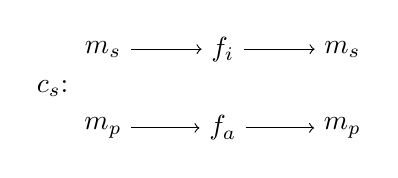
\begin{tikzpicture}[x=.8cm, y=.5cm]

%speaker strategies
\node at (-0.1,6) {$c_s$:};

\node at (0.7,7) (tc){$m_s$};
\node at (0.7,5) (tg){$m_p$};

\node at (2.6,7) (mc){$f_{i}$};
\node at (2.6,5) (mg){$f_{a}$};

\node at (4.5,7) (ac){$m_s$};
\node at (4.5,5) (ag){$m_p$};

\path[->] (tc) edge [right] (mc);
\path[->] (tg) edge [right] (mg);

\path[->] (mc) edge [right] (ac);
\path[->] (mg) edge [right] (ag);

\end{tikzpicture}
\end{minipage}
\begin{minipage}{51mm}	
\centering    
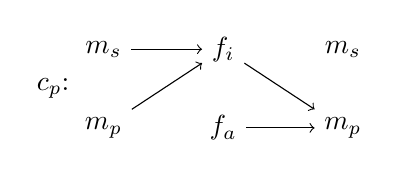
\begin{tikzpicture}[x=.8cm, y=.5cm]

%speaker strategies
\node at (-0.1,6) {$c_p$:};

\node at (0.7,7) (tc){$m_s$};
\node at (0.7,5) (tg){$m_p$};

\node at (2.6,7) (mc){$f_{i}$};
\node at (2.6,5) (mg){$f_{a}$};

\node at (4.5,7) (ac){$m_s$};
\node at (4.5,5) (ag){$m_p$};

\path[->] (tc) edge [right] (mc);
\path[->] (tg) edge [right] (mc);

\path[->] (mc) edge [right] (ag);
\path[->] (mg) edge [right] (ag);

\end{tikzpicture}
\end{minipage}


\caption{The two strategy pairs of an optional progressive grammar: for contextual cue $c_s$ the strategy pair forms a signaling equilibrium, whereas for contextual cue $c_p$ it forms a  pooling equilibrium.}
\label{fig:s2h1-sigsys}
\end{figure}

Another strategy for the Imperfective Game is given in \figref{fig:s10h5-sigsys}. Here  the behavior differs from the former strategy only when context $c_p$ is given (right). Here speaker and hearer behave exactly the same as they did for the context $c_s$. This strategy pair represents a categorical progressive grammar, such as in \ili{English}, where one form is exclusively used for phenomenal meanings (in other words, a categorical progressive marker), whereas the other form is exclusively used for structural meanings. A very important difference between both systems is that the former is partially context-dependent, since interlocutors behave differently in different contexts, whereas the second one is context-independent. A categorical progressive system such as \ili{English} needs much fewer contextual cues for expressing and understanding an ongoing event (phenomenal meaning), than an emergent progressive system, such as \ili{Spanish}.

\begin{figure}[t]
\centering
\begin{minipage}{51mm}	
\centering  
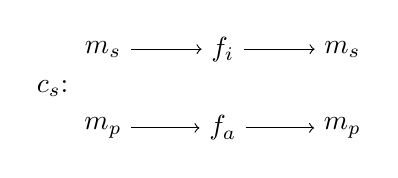
\begin{tikzpicture}[x=.8cm, y=.5cm]

%speaker strategies
\node at (-0.1,6) {$c_s$:};

\node at (0.7,7) (tc){$m_s$};
\node at (0.7,5) (tg){$m_p$};

\node at (2.6,7) (mc){$f_{i}$};
\node at (2.6,5) (mg){$f_{a}$};

\node at (4.5,7) (ac){$m_s$};
\node at (4.5,5) (ag){$m_p$};

\path[->] (tc) edge [right] (mc);
\path[->] (tg) edge [right] (mg);

\path[->] (mc) edge [right] (ac);
\path[->] (mg) edge [right] (ag);

\end{tikzpicture}
\end{minipage}
\begin{minipage}{51mm}	
\centering    
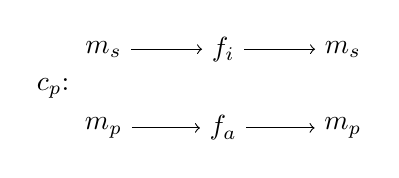
\begin{tikzpicture}[x=.8cm, y=.5cm]

%speaker strategies
\node at (-0.1,6) {$c_p$:};

\node at (0.7,7) (tc){$m_s$};
\node at (0.7,5) (tg){$m_p$};

\node at (2.6,7) (mc){$f_{i}$};
\node at (2.6,5) (mg){$f_{a}$};

\node at (4.5,7) (ac){$m_s$};
\node at (4.5,5) (ag){$m_p$};

\path[->] (tc) edge [right] (mc);
\path[->] (tg) edge [right] (mg);

\path[->] (mc) edge [right] (ac);
\path[->] (mg) edge [right] (ag);

\end{tikzpicture}
\end{minipage}

\caption{The two strategy pairs of a categorical progressive grammar: the strategy pair forms the same signaling equilibrium for both contextual cues, therefore being context independent.}
\label{fig:s10h5-sigsys}
\end{figure}

A very important concept for the study of signaling games is the \emph{signaling equilibrium}: 
a one-to-one mapping between forms and meanings. In other words, signaling equilibria are strategy pairs for which the speaker uses a different form for each meaning, and the hearer behaves according to the exact mirror image. Signaling equilibria have very important properties
\citep[cf.][]{jaeger08stability}. Note that the left strategy pair in \figref{fig:s2h1-sigsys} is a signaling equilibrium, as are both strategy pairs in \figref{fig:s10h5-sigsys}. On the other hand, the right strategy pair in \figref{fig:s2h1-sigsys} is not a signaling equilibrium. It does not guarantee perfect information transmission, but at least it guarantees partial information transmission: interlocutors can  communicate meaning $m_p$ via form $f_{i}$. Such systems of partial transmission are also called \emph{pooling equilibria}.

Note that the set of all possible strategies is called the \emph{strategy space}, with $S$ being the speaker's strategy space, and $H$ being the hearer's strategy space. When we model a grammatical system via a signaling game, it is important to understand the dimensions of the strategy spaces for at least one reason: the models can readily produce \emph{combinatorial explosions}. As we will see for the Case Game, the strategy space can be huge and often impossible to handle and analyze. Understanding the strategy space helps to find reasonable ways to reduce it to a number of strategies that can be dealt with.\footnote{``Reasonable ways'' refer, above all, to the detection and deletion of strategies which are admittedly logically possible, but e.g,~are invalid with the grammatical system, or are at least highly unlikely to emerge in the context of the given grammar game. Such strategies are supposed to be an alternative that a rational agent would never consider using in the first place. An example would be to use an ergative marker for the accusative case (or vice versa), as discussed in the next section. It is important to note that space reduction is not supposed to be a process conducted by language users, but a preselection made by the modeler to obtain only those strategies that are reasonable candidates to be considered by language users at all.} In what follows I will discuss the strategy spaces of the Case Game and the Imperfective Game, and possible methods for \emph{strategy space reduction}.

\subsubsection{Strategy space of the Case Game}

The dimensions of the strategy space of a signaling game can be easily computed by the number of meanings $|M|$, the number of forms $|F|$, and the number of contextual cues $|C|$. Since a speaker strategy is defined as a function from the space $C \times M$ to the space $F$, it entails $|F|^{(|C| \cdot |M|)}$ different speaker strategies. Since the Case Game has $|F|=7$ forms, $|M| = 2$ meanings, and $|C|=4$ contextual cues, it entails $7^{(4 \cdot 2)}$ speaker strategies, which amounts to almost 6 million possibilities. Similarly, the number of hearer strategies is given by $|M|^{(|C| \cdot |F|)} = 2^{28}$, which amounts to almost 270 million possibilities. The number of strategy pairs is computed as a product of those two numbers, resulting in a number of 16 digits! It should be clear from these numbers 
that it would be impossible to work with the full strategy space $S \times H$ of the Case Game.

Jäger reduced the space of speaker strategies in multiple ways. First, he joined strategies that have the same case marking structure, but only differ in word order. For example, the usage of form $f_{ez}$ for meaning $m_{AO}$ and the usage of form $f_{ze}$ for meaning $m_{OA}$ both describe the same way of case marking, namely marking the agent with an ergative marker, and zero-marking the object. Furthermore, he also excluded strategies that would mark the agent as accusative and/or the object as ergative. Additionally, he used the concept of strict strategy domination \citep[cf.][]{Watson2008} to eliminate so-called dominated strategies.\footnote{I will not go into greater detail with respect to the ways in which strategies can be reduced, since it would exceed this study's purpose. 
Yet, this case should make sense for the problem of combinatorial explosions and hint at the fact that there are elaborate ways to reduce the strategy space.} This treatment rules out strategies, which e.g.~always mark both NPs, such as using $f_{ea}$ for meaning $m_{AO}$, and using form $f_{ae}$ for meaning $m_{OA}$ among all contexts.

This whole process reduces the space of speaker strategies from almost six million to ten strategies! These strategies can be described as follows:

\begin{description}
\item[$s_1$:] $\forall c \in C:$ $(c,m_{AO}) \rightarrow f_{ez}$ (always $e$-mark the agent)
\item[$s_2$:] $\forall c \in C:$ $(c,m_{AO}) \rightarrow f_{za}$ (always $a$-mark the object)
\item[$s_3$:] $(c_{nn},m_{AO}) \rightarrow f_{zz}$; $(c_{pp}, m_{AO}) \rightarrow f_{ea}$; $(c_{pn},m_{AO}) \rightarrow f_{ez}$; $(c_{np},m_{AO}) \rightarrow f_{za}$ (always mark the prominent NP, never the non-prominent NP) 
\item[$s_4$:] $(c_{nn}, m_{AO}) \rightarrow f_{ea}$; $(c_{pp},m_{AO}) \rightarrow f_{zz}$; $(c_{pn},m_{AO}) \rightarrow f_{za}$; $(c_{np},m_{AO}) \rightarrow f_{ez}$ (always mark the non-prominent NP, never the prominent NP) 
\item[$s_5$:] $(c_{nn},m_{AO}) \rightarrow f_{ez}$; $(c_{pp},m_{AO}) \rightarrow f_{za}$; $(c_{pn},m_{AO}) \rightarrow f_{zz}$; $(c_{np},m_{AO}) \rightarrow f_{ea}$ ($e$-mark the non-prominent agent; $a$-mark the prominent object) 
\item[$s_6$:] $(c_{nn},m_{AO}) \rightarrow f_{zz}$; $(c_{pp},m_{AO}) \rightarrow f_{ez}$; $(c_{pn},m_{AO}) \rightarrow f_{ez}$; $(c_{np}, m_{AO}) \rightarrow f_{zz}$ ($e$-mark the prominent agent)
\item[$s_7$:] $(c_{nn},m_{AO}) \rightarrow f_{ez}$; $(c_{pp},m_{AO}) \rightarrow f_{zz}$; $(c_{pn},m_{AO}) \rightarrow f_{zz}$; $(c_{np},m_{AO}) \rightarrow f_{ez}$ ($e$-mark the non-prominent agent) 
\item[$s_8$:] $(c_{nn},m_{AO}) \rightarrow f_{zz}$; $(c_{pp},m_{AO}) \rightarrow f_{za}$; $(c_{pn},m_{AO}) \rightarrow f_{zz}$; $(c_{np},m_{AO}) \rightarrow f_{za}$ ($a$-mark the prominent object)
\item[$s_9$:] $(c_{nn},m_{AO}) \rightarrow f_{za}$; $(c_{pp},m_{AO}) \rightarrow f_{zz}$; $(c_{pn},m_{AO}) \rightarrow f_{za}$; $(c_{np},m_{AO}) \rightarrow f_{zz}$ ($a$-mark the non-prominent object)
\item[$s_{10}$:] $\forall c \in C:$ $(c,m_{AO}) \rightarrow f_{zz}$ (no case marking)
\end{description}


The space of hearer strategies can also be drastically reduced. First, note that whenever a hearer receives a form that is not $f_{zz}$, he can easily detect agent and object. If one of the NPs is $e$-marked, it must be the agent, whereas if one of the NPs is $a$-marked, it must be the object. Therefore, the hearer can use the ultimate strategy: if one NP is $e$-marked, construe it as agent and the other NP as object; if one NP is $a$-marked, construe it as object, and the other NP as agent. This strategy works for all forms, except for $f_{zz}$, as displayed in \figref{strat:hearer-case} (left).

\begin{figure}[t]
\begin{minipage}{5cm}
\centering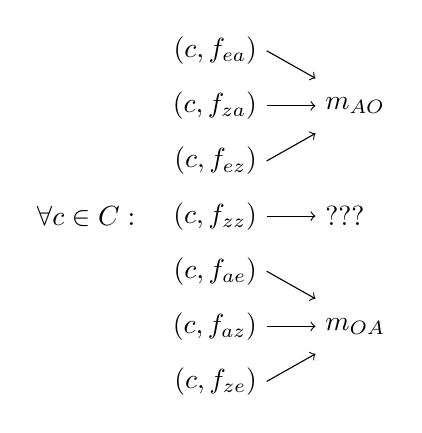
\begin{tikzpicture}[x=.31cm, y=.35cm]
%receiver strategies
\node at (-4,6) {$\forall c \in C:$};
\draw [->](3.4,12) node[left]{$(c, f_{ea})$} -> (5.4,11) node[right]{};
\draw [->](3.4,10) node[left]{$(c, f_{za})$} -> (5.4,10) node[right]{$m_{AO}$};
\draw [->](3.4,8) node[left]{$(c, f_{ez})$} -> (5.4,9) node[right]{};
\draw [->](3.4,6) node[left]{$(c, f_{zz})$} -> (5.4,6) node[right]{???};
\draw [->](3.4,4) node[left]{$(c, f_{ae})$} -> (5.4,3) node[right]{};
\draw [->](3.4,2) node[left]{$(c, f_{az})$} -> (5.4,2) node[right]{$m_{OA}$};
\draw [->](3.4,0) node[left]{$(c, f_{ze})$} -> (5.4,1) node[right]{};
\end{tikzpicture}
\end{minipage}\hfill\begin{minipage}{7cm}
\centering    
\begin{description}
\item[$h_1$:] $\forall c \in C:$ $(c,f_{zz}) \rightarrow m_{AO}$ (first NP is agent, or subject before object)
\item[$h_2$:] $(c_{nn},f_{zz}) \rightarrow m_{AO}$; $(c_{pp},f_{zz}) \rightarrow m_{AO}$; $(c_{pn},f_{zz}) \rightarrow m_{AO}$; $(c_{np},f_{zz}) \rightarrow m_{OA}$ (more prominent NP is agent) 
\item[$h_3$:] $(c_{nn},f_{zz}) \rightarrow m_{AO}$; $(c_{pp},f_{zz}) \rightarrow m_{AO}$; $(c_{pn},f_{zz}) \rightarrow m_{OA}$; $(c_{np},f_{zz}) \rightarrow m_{AO}$ (more prominent NP is object)
\item[$h_4$:] $\forall c \in C:$ $(c,f_{zz}) \rightarrow m_{OA}$ (first NP is object, or object before subject)
\end{description}
\end{minipage}
\caption{\emph{Left}: the ultimate hearer strategy is completely context-independent and works as long as at least one NP is case marked, but it does not have an answer when the hearer receives $f_{zz}$. \emph{Right}: the four substrategies that use either word order information ($h_1$, $h_4$) or prominence information ($h_2$, $h_3$) to discriminate between meanings.}
\label{strat:hearer-case}
\end{figure}

To handle the $f_{zz}$-situation, Jäger introduced four substrategies that deal with this case in different ways: $h_1$: the first NP is the agent, (ii) $h_2$: the more prominent NP is agent, (iii) $h_3$: the more prominent NP is object, and (iv) $h_4$: the first NP is object, as shown in \figref{strat:hearer-case} (right). Note that $h_1$ and $h_4$ use word order to discriminate between meanings, whereas $h_2$ and $h_3$ use prominence information. Note also that $h_2$ and $h_3$ additionally use word order (agent before object), when both NPs have the same prominence level. In this way, Jäger finally reduced the space of almost 270 million hearer strategies to four! Therefore, the resulting strategy spaces of the Case Game contain 10 speaker and 4 hearer strategies. In the next subsection, I will show that the Imperfective Game similarly does not entail such a combinatorial explosion.


\subsubsection{Strategy space of the Imperfective Game}

Since the Imperfective Game has $|F|=2$ forms, $|M| = 2$ meanings, and $|C| = 2$ contextual cues, it entails $2^{(2 \cdot 2)}= 16$ speaker strategies, as well as $2^{(2 \cdot 2)}= 16$ hearer strategies.  The number of strategy pairs is therefore $16 \cdot 16 = 256$. Note that unlike Jäger's game, Deo's game amounts to a total number of strategies that can be dealt with computationally.\footnote{See \citet{muehlenberndEnke_2017} for a computational study that incorporates the whole strategy space of Deo's Imperfective Game.} Nevertheless, Deo also reduced the strategy space by focusing on those strategies that are assumed to represent the different stages of the grammars of the progressive-imperfective grammaticalization path (see \sectref{sec:intro:prog}). The four relevant speaker strategies are as follows:

\begin{description}%[itemsep=.5pt]
\item[$s_I$:] $\forall c \in C, \forall m \in M:$ $(c,m) \rightarrow f_{i}$ (always use the imperfective marker)
\item[$s_O$:] $(c_{p},m_{p}) \rightarrow f_{i}$; $(c_{p},m_{s}) \rightarrow f_{i}$; $(c_{s},m_{p}) \rightarrow f_{a}$; $(c_{s},m_{s}) \rightarrow f_{i}$ (use the additional marker $f_a$ which is optional for $m_p$ in case when it is not supported by the contextual cue, else use $f_i$) 
\item[$s_C$:] $\forall c \in C:$ $(c,m_{s}) \rightarrow f_{i}$, $(c,m_{p}) \rightarrow f_{a}$ (use both markers categorically, with $f_i$ for $m_s$ and $f_a$ for $m_p$)
\item[$s_A$:] $\forall c \in C, \forall m \in M:$ $(c,m) \rightarrow f_{a}$ (always use the additional marker)
\end{description}

\noindent Furthermore, the three relevant hearer strategies are as follows:

\begin{description}
\item[$h_{X}$:] $\forall c_i \in C, \forall f \in F:$ $(c_i,f) \rightarrow m_{i}$ (construe context dependence, choose the meaning that fits the context)
\item[$h_O$:] $(c_{p},f_{i}) \rightarrow m_{p}$; $(c_{p}, f_{a}) \rightarrow m_{p}$; $(c_{s}, f_{i}) \rightarrow m_{s}$; $(c_{s}, f_{a}) \rightarrow m_{p}$ (construe meaning according to the context, except when additional marker $f_a$ is used in a non-supported context: hearer pendant to $s_O$) 
\item[$h_C$:] $\forall c \in C:$ $(c, f_i) \rightarrow m_s$, $(c, f_a) \rightarrow m_p$ (construe both markers categorically, with $m_s$ for $f_i$ and $m_p$ for $f_a$)
\end{description}

\noindent Now, the four stages can be represented by the following strategy pairs:

\begin{description}
\item[zero-progressive (ZP) using solely $f_i$:] $(s_I,h_X)$
\item[emergent-progressive (EP):] $(s_O,h_O)$
\item[categorical-progressive (CP):] $(s_C,h_C)$
\item[zero progressive (ZP$^*$) using solely $f_a$:] $(s_A,h_X)$
\end{description}


\subsection{Step 4: Utility functions and the EU table}
\label{sec4-utility}

One fundamental aspect of game-theoretic models is the definition of a utility function. The utility function maps strategic behavior to a numerical value which represents the preferences of the players. In a signaling game, both players -- speaker and hearer -- prefer successful communication over non-successful communication; therefore, an outcome of the former kind must result in a higher payoff for both than one of the latter. The success of communicating a particular meaning $m \in M$, whereby the speaker uses strategy $s$ and the hearer uses strategy $h$, can be defined by the following $\delta_m$-function:

$$\delta_m(s,h) = \begin{cases}
1 & \text{iff } h(s(m)) = m\\
0 &\text{otherwise} 
\end{cases}$$

$\delta_m$ simply returns 1 when the hearer construes the meaning the speaker wants to communicate, and 0 if not. Note that this is the original definition by \citet{Jaeger07}. In his model, he did not explicitly define a context space, but integrated it as part of the meaning space. By integrating the contextual space, communicative success can be defined by a $\delta_{c,m}$-function in the following way:

$$\delta_{c,m}(s,h) = \begin{cases}
1 & \text{iff } h(c,s(c,m)) = m\\
0 &\text{otherwise} 
\end{cases}$$

Note that the $\delta_{c,m}$-function determines whether a particular pair of speaker strategy $s$ and hearer strategy $h$ is successful (1) or not (0), given the particular situation that the meaning is $m$ and the context is $c$. To estimate a comprehensive utility value for a speaker strategy $s$ and a hearer strategy $h$, both have to be defined over the whole meaning space and over the whole context space. Such a utility is called \emph{expected utility} $EU$ and is defined as the average communicative success over all contexts $c \in C$ and meanings $m \in M$, by taking prior probability $P(m|c)$ into consideration. Therefore the \emph{hearer expected utility} $EU_h$ for using strategy $h$ against strategy $s$ is defined as follows:

$$EU_h(s,h) = \sum_{c \in C}  \sum_{m \in M} P(m|c) \cdot \delta_{c,m}(s,h)$$

\noindent The \emph{speaker expected utility} $EU_s$ is defined in the same way by additionally incorporating the costs $\mathcal{K}$ that the speaker has to pay with respect to her strategy: 

$$EU_s(s,h) = \sum_{c \in C} \sum_{m \in M} P(m|c) \cdot (\delta_{c,m}(s,h) - k  \cdot \mathcal{K})$$

\noindent Here $\mathcal{K}$ is a placeholder for either a form-dependent cost function $K_f(s(c,m))$ based on the costs of each form $f=s(c,m)$ that is used in the speaker strategy $s$, or for a strategy-dependent cost function $K_s(s)$ based on the costs of the speaker strategy  $s$ itself.
Furthermore, the parameter $k$ is an additional factor, with $0 \leq k \leq 1$, which specifies the  speaker's priorities: if $k$ is low, communicative success is more important than minimal effort, and vice versa. In the Case Game, $k$ represents how costly case morphology is. For example, one can say that case marking is more useful in languages with free word order than  in those with fixed word order. Therefore, it is relatively more costly to have case marking in the latter case, where it is less needed for disambiguation \citep[see][85 for a more detailed discussion]{Jaeger07}. All in all, the higher $k$ is, the more additional options a language has to disambiguate between meanings, and the less needed and therefore more costly grammatical marking is.

Given these functions, we can compute the \emph{expected utility} (EU) table, which represents the expected utility value of both players for each combination of speaker and hearer strategy. In the following section I will present the EU tables of the Case Game and of the Imperfective Game.

\subsubsection{EU tables of the Case Game}

Grammar games as defined here entail an infinite number of EU tables. Each depends on the $k$-value of the speaker utility function $EU_s$, since this parameter changes the utility values of the speaker. \tabref{EU_Case} shows the EU tables for a relatively low $k$-value of 0.1 (left) and a median one of $0.45$ (right). Note that these tables solely contain the expected utility values of the speaker ($EU_s$), but -- as \citet{Jaeger07} argued -- since the relative utilities between speaker and hearer expected utility do not differ for the hearer, it suffices to consider only the expected utilities of the speaker without changing the qualitative results of evolutionary analysis.

\begin{table}
\begin{subtable}{.5\textwidth}\centering
\caption{$k=0.1$}
\begin{tabular}{lllll} 
\lsptoprule
 & \multicolumn{1}{c}{$h_1$} & \multicolumn{1}{c}{$h_2$} & \multicolumn{1}{c}{$h_3$} & \multicolumn{1}{c}{$h_4$}  \\\midrule
$s_1$ & 0.9  &  0.9  & 0.9 & 0.9  \\
$s_2$ & 0.9  &  0.9  & 0.9 & 0.9  \\
$s_3$ & 0.85  &  0.85  & 0.85 & 0.85  \\
$s_4$ & 0.81  &  0.81  & 0.81 & 0.81  \\
$s_5$ & 0.61  &  \textbf{0.97}  & 0.26 & 0.61  \\
$s_6$ & 0.86  &  0.86  & 0.87 & 0.86  \\
$s_7$ & 0.54  &  0.89  & 0.54 & 0.54  \\
$s_8$ & 0.59  &  0.94  & 0.59 & 0.59  \\
$s_9$ & 0.81  &  0.81  & 0.82 & 0.81  \\
$s_{10}$ & 0.5  &  0.85  & 0.15 & 0.5  \\\lspbottomrule
\end{tabular}
\end{subtable}\begin{subtable}{.5\textwidth}\centering
\caption{$k=0.45$}
\begin{tabular}{lllll} 
\lsptoprule
 & \multicolumn{1}{c}{$h_1$} & \multicolumn{1}{c}{$h_2$} & \multicolumn{1}{c}{$h_3$} & \multicolumn{1}{c}{$h_4$}  \\\midrule
$s_1$ & 0.55  &  0.55  & 0.55 & 0.55  \\
$s_2$ & 0.55  &  0.55  & 0.55 & 0.55  \\
$s_3$ & 0.458  &  0.458  & 0.458 & 0.458  \\
$s_4$ & 0.507  &  0.507  & 0.507 & 0.507  \\
$s_5$ & 0.507  &  0.863  & 0.151 & 0.507  \\
$s_6$ & 0.545  &  0.538  & \textbf{0.553} & 0.545  \\
$s_7$ & 0.505  &  0.861  & 0.148 & 0.505  \\
$s_8$ & 0.510  &  \textbf{0.867}  & 0.154 & 0.51  \\
$s_9$ & 0.539  &  0.531  & 0.547 & 0.539  \\
$s_{10}$ & 0.5  &  0.849  & 0.152 & 0.5  \\\lspbottomrule
\end{tabular}
\end{subtable}
\caption{EU tables (only $EU_s$ values) of the Case Game with $k=0.1$ (left) and $k=0.45$ (right). The bold numbers are the utility values of strategy pairs that are evolutionarily stable strategies.\label{EU_Case}}
\end{table}


Importantly, these EU tables are the object of investigation when we want to study the stability of grammars. I will be more concrete in \sectref{sec:EGT} when I introduce EGT tools for analyzing such EU tables. Then I will also introduce the fundamental concept of an \emph{evolutionarily stable strategy} (ESS). As a simple heuristic, for asymmetric EU tables (such as those of \tabref{EU_Case}), evolutionary stable strategies can easily be located by finding utility values that are the unique maximum in their row and column. In \tabref{EU_Case}, the strategy pairs that form ESSs are marked in bold. Here, the strategy pair $(s_5,h_2)$ is an ESS when $k$ is relatively low (left table). Note that this strategy pair represents a DSOM grammar, which is a combination of differential subject and object marking and very common in \ili{Australian} languages \citep[cf.][]{Dixon1994}. Furthermore, when $k$ is higher (right table), then, e.g., the strategy pair $(s_8,h_2)$ is an ESS, which represents a DOM grammar, such as \ili{English}.

\subsubsection{EU tables of the Imperfective Game}

The Imperfective Game also produces multiple EU tables which are dependent on the $k$-value. \tabref{EU_Imp} shows the table for $k=0.1$ (left) and $k=0.45$ (right). Note that solely depicting the speaker utility is sufficient to study the characteristics -- for the same reason as for the Case Game. As highlighted, the only ESS in both tables is the strategy pair $(s_C, h_C)$: the categorical progressive system. This is also the only signaling equilibrium of the reduced strategy space (cf.~\figref{fig:s10h5-sigsys}). 

\begin{table}
\begin{subtable}{.5\textwidth}\centering
\caption{$k=0.1$}
\begin{tabular}{lllll} 
\lsptoprule
 & \multicolumn{1}{c}{$h_X$} & \multicolumn{1}{c}{$h_O$} & \multicolumn{1}{c}{$h_C$}  \\\midrule
$s_I$   & 0.9  &  0.9  & 0.5   \\
$s_O$ & 0.8  &  0.85  & 0.45   \\
$s_C$ & 0.8  &  0.85  & \textbf{0.9}   \\
$s_A$ & 0.9  &  0.5  & 0.5   \\\lspbottomrule
\end{tabular}
\end{subtable}\begin{subtable}{.5\textwidth}\centering
\caption{$k=0.45$}
\begin{tabular}{lllll}
\lsptoprule
 & \multicolumn{1}{c}{$h_X$} & \multicolumn{1}{c}{$h_O$} & \multicolumn{1}{c}{$h_C$}  \\\midrule
$s_I$   & 0.9  &  0.9  & 0.5   \\
$s_O$ & 0.45  &  0.5  & 0.1   \\
$s_C$ & 0.45  &  0.5  & \textbf{0.55}   \\
$s_A$ & 0.9  &  0.5  & 0.5   \\
\lspbottomrule
\end{tabular}
\end{subtable}
\caption{EU tables (only $EU_s$ values) of the Imperfective Game with $k=0.1$ (left) and $k=0.45$ (right). The bold numbers are the utility values of strategy pairs that are evolutionary stable strategies.\label{EU_Imp}}
\end{table}

To make a more elaborate analysis of grammar games, we can use concepts and tools from EGT which will be introduced in the next section. But just to wrap up at this point: the goal of the modeling is to define a signaling game that represents a particular grammatical domain. From the model, we can calculate EU tables, 
%deduce From this, we can calculate EU tables -- as happened in this section -- 
which are the objects of investigation for EGT analyses. 
%investigation in terms of EGT. 
A schematic sketch of the modeling process is depicted in \tabref{sceme-model}.


\begin{table}\small
\begin{subtable}{\textwidth}
\caption{Step 1:  Definition of meaning, form, and context space}
\begin{tabularx}{\textwidth}{Qp{.25\textwidth}Q}
\lsptoprule
& Case Game & Imperfective Game \\\midrule
meaning space & agent/object &  struct./phen.~reading   \\
form space & acc./erg./zero marker & imperf./additional marker   \\
context space &  prominence inf. & cue for struct./phen.~reading \\\lspbottomrule
\end{tabularx}
\end{subtable}\medskip\\
\begin{subtable}{\textwidth}
\caption{Step 2: Defining prior probabilities and cost function}
\begin{tabularx}{\textwidth}{Qp{.25\textwidth}Q}
\lsptoprule
& Case Game & Imperfective Game \\\midrule
source for prior $P(m|c)$ & corpus data & ad-hoc values   \\
type of cost function & form-related & strategy-related   \\
cost function factors in: &  number of markers & number of forms used in strategy \\\lspbottomrule
\end{tabularx}
\end{subtable}\medskip\\
\begin{subtable}{\textwidth}
\caption{Step 3: Strategy space reduction}
\begin{tabularx}{\textwidth}{Qp{.25\textwidth}Q}
\lsptoprule
& Case Game & Imperfective Game \\\midrule
speaker strategy reduction & $\sim 6$ million $\rightarrow 10$ & $16 \rightarrow 4$   \\
hearer strategy reduction & $\sim 270$ million $\rightarrow 4$ & $16 \rightarrow 3$   \\\lspbottomrule
\end{tabularx}
\end{subtable}\medskip\\
\begin{subtable}{\textwidth}
\caption{Step 4: EU table computation}
\begin{tabularx}{\textwidth}{Qp{.25\textwidth}Q}
\lsptoprule
& Case Game & Imperfective Game \\\midrule
EU table ($k=0.1$) & see \tabref{EU_Case} (left) & see \tabref{EU_Imp} (left)   \\
EU table ($k=0.45$)  & see \tabref{EU_Case} (right) & see \tabref{EU_Imp} (right)  \\\lspbottomrule
\end{tabularx}
\end{subtable}
\caption{Schematic representation of the modeling process. Step 1: Define the relevant spaces of the grammatical domain. Bring to mind what is core information for the coding system under investigation to set up the form and meaning space. Then think of particular domain(s) that provide contextual cues, such as prominence information, (cf.~Case Game) or set up ad-hoc  contexts (cf.~Imperfective Game). Step 2: Define the relationship between context and meaning in the form of a prior probability function, that might be determined by empirical data (Case Game) or as ad-hoc values (Imperfective Game). Then define a cost function with respect to the complexity of the grammar, which can be form-related (Case Game) or strategy-related (Imperfective Game). Step 3: Compute the number of speaker and hearer strategies and under certain conditions -- such as combinatorical explosions (cf.~Case Game) -- reduce the space in reasonable ways. Step 4: Given the set of (reduced) strategies, compute the EU tables via the speaker and hearer expected utility function $EU_s$ and $EU_h$, respectively. }
\label{sceme-model}
\end{table}


\section{Evolutionary Game Theory: Concepts and tools}
\label{sec:EGT}
 
Languages or grammars can be seen as self-replicating systems, which are subject to variation and selection. 
Linguistic selection is most certainly guided by factors that are functional, cognitive, and social as well. While \emph{Epistemic Game Theory} focuses on the cognitive processes of agents, we will look at the other side of the coin using \emph{Evolutionary Game Theory} (EGT). EGT mainly abstracts from the individual agent and her specific cognitive processes guiding decisions, and considers the dynamics of populations instead. This step of abstraction is in some aspects very valuable, since due to its low complexity it enables a mathematical analysis of the population dynamics of the game-model to be performed; on the other hand it does not allow for e.g.~incorporating agent-based aspects in a very fine-grained way, such as in the case of many social or cognitive factors. Yet EGT is very useful for studying the role of functional factors in the cultural evolution of grammars.  
 
 
EGT was originally developed by theoretical biologists \citep{Maynard73,Maynard82} to formalize neo-Darwinian concepts of evolution. The idea is that the interactions between different members of a population can be modeled in a game-theoretic sense. Here, the population members are represented by strategies of a game, and a strategy's average payoff represents its fitness. Evolutionary dynamics ensure that a higher fitness generally entails a higher chance of reproduction. 
More precisely, evolutionary dynamics determines the change of the population's configuration -- the \emph{population state}, that is, the proportions of all strategies in the population -- in the following way: the greater/less the relative fitness of a strategy, the more its proportion increases/decreases. This can, for example, lead to situations where one single strategy conquers the whole population, whereas all competitors die out. 

Note that I will introduce EGT concepts that are designed for 2-player games, since I believe that most instances of language use and communication are 2-person situations between a speaker and a hearer (as also represented by the standard definition of a signaling game). However, these concepts can also be generalized to n-player situations \citep[cf.][]{Hofbauer_2003,Veelen_2011}. Furthermore, the evolutionary dynamics I will introduce are designed for \emph{infinite} population scenarios with a \emph{homogeneous} structure where every member interacts with every other member with the same frequency. This is of course an unrealistic assumption when it comes to human societies that are finite and interact in social network structures, but it simplifies the formal analysis immensely. Nonetheless, there exists plenty of literature that studies  evolutionary dynamics in finite and \emph{heterogeneous} populations, from classical game-theoretic scenarios \citep[cf.][]{Nowak_1992,Taylor_2004,Lieberman_2005} to signaling games \citep[cf.][]{Skyrms10,Huttegger11,Muehlenbernd_14,Muehlenbernd2021,Muehlenbernd2022} and more language-specific mechanisms of cultural evolution \citep[cf.][]{Baxter_2006,Fagyal10,Blythe_2012}.


\subsection{Tool 1: How to compute symmetric games}

Note that the EU tables of the Case Game and the Imperfective Game (Tables~\ref{EU_Case} and~\ref{EU_Imp}) are non-symmetric: the row strategies differ from the column strategies, since the former are speaker strategies and the latter are hearer strategies. Such an \emph{asymmetric game} is generally represented by a 2-population model in terms of EGT (one population represents speaker strategies, the other, hearer strategies). It is often useful to analyze them as \emph{symmetric games} (as 1-population models). When we  deduce symmetric games from asymmetric signaling games, we do not consider speaker strategies $s \in S$ and hearer strategies $h \in H$ as single options anymore, but as strategy pairs $(s,h) \in S \times H$ instead. An entry of such a symmetric game table is given by the expected utility value $EU_p((s_i,h_i),(s_j,h_j))$, defined as how well a strategy pair $(s_i,h_i)$ works with another strategy pair $(s_j,h_j)$:

\[EU_p((s_i,h_i),(s_j,h_j)) =  \frac{EU_s(s_i,h_j) + EU_h(s_j,h_i)}{2}\]

Note that for a given asymmetric game with dimension $n \times m$, the corresponding symmetric game has the dimension $(n\cdot m)\times (n\cdot m)$. For example, the EU table of the Case Game has dimension $10 \times 4$, and its symmetric pendant amounts to a $40 \times 40$ game table. Accordingly, the dimensions of the  game table of the Imperfective Game  changes from $4 \times 3$ to $12 \times 12$. 
To present an example, in her analysis \citet{Deo_2015} used a subgame\footnote{A subgame can be computed by selecting a subset of the original strategy set(s) and the respective utility values.} of the symmetric game table of the Imperfective Game by solely paying attention to those strategy pairs that constitute the different stages of the progressive-imperfective grammaticalization path. The EU table of the subgame is given in \tabref{EU_Imp_sym}. 

\begin{table}
\begin{tabular}{l llll} 
\lsptoprule
 & \multicolumn{1}{c}{$(s_I, h_X)$} & \multicolumn{1}{c}{$(s_O, h_O)$} & \multicolumn{1}{c}{$(s_C, h_C)$} &  \multicolumn{1}{c}{$(s_A, h_X)$}\\\midrule
$(s_I, h_X)$   & 0.9  &  0.9  & 0.7 & 0.9  \\
$(s_O, h_O)$ & 0.8  &  0.85  & 0.65 & 0.6   \\
$(s_C, h_C)$ & 0.6  &  0.65  & \textbf{0.9} & 0.6   \\
$(s_A, h_X)$ & 0.9  &  0.7  & 0.7 & 0.9   \\
\lspbottomrule
\end{tabular}
\caption{Symmetric EU table of strategy pairs for the Imperfective Game (only row player's $EU_p$ values) with $k=0.2$, restricted to four strategy pairs. The bold number marks the only ESS of the game.\label{EU_Imp_sym}}
\end{table}

Note that for a symmetric utility table, it is sufficient to depict solely the row player's utilities, since the column player's utilities are the same as those of the row player when mirrored across the northwest-to-southeast diagonal.

In  the next section, I will use subgames of those symmetric game tables to better illustrate an important concept in EGT: the \emph{replicator dynamics}.


\subsection{Tool 2: The replicator dynamics}

The replicator dynamics in its general specification is a dynamics that models replication in populations, one example being biological reproduction. It is defined for an infinite population, where its members are programmed for a certain strategy and interact under totally random pairings. 
The \emph{fitness} of a strategy is defined by its accumulated utility value over the interactions, and the average number of a member's offspring is proportional to the fitness of her strategy.
For the formal definition of the replicator dynamics, I will here restrict myself to symmetric games (see \citealt{HofbauerSigmund1988} for asymmetric games). Before defining the replicator dynamics, I have to introduce some further notions.

A \emph{population state}  represents the proportions of the population's members using particular strategies. More precisely, let $x_i \in \mathbb{R}$ be the proportion of a population using strategy $g_i \in G$.\footnote{I use here and any time afterwards the label $g$ for a strategy in general (and $G$ for the set of strategies, appropriately). Note that in the case of a grammar game, $g$ can stand for a speaker strategy $s$, a hearer strategy $h$, or a pair of both, depending on the type of the game table.} Now, a population state for $n$ strategies can be presented as a vector $\textbf{x} \in \mathbb{R} ^n$, with $\forall x_i$ in $\textbf{x}: 0 \leq x_i \leq 1$, and $\sum_{i=1}^n x_i= 1$.
Given a population state $\textbf{x}$, the \emph{fitness} $f_i$ of strategy $g_i$ is defined as $f_i(\textbf{x}) = \sum_{j=1}^n x_j EU(x_i,x_j)$, where $EU$ is the game's (expected) utility function. The fitness represents the average score of a strategy against all other strategies in the population with respect to population state $\textbf{x}$. The \emph{average fitness} $\phi$ of the whole population can now be defined as $\phi(\textbf{x}) = \sum_{i=1}^n x_i f_i(\textbf{x})$, which represents the average over all strategies' fitness values with respect to population state $\textbf{x}$.

The replicator dynamics defines how these population states change over time: the proportion of the population playing a strategy $g_i$ in the next generation depends on (i) its proportion $x_i$ of the current generation and (ii) its success in the form of overall utility $f_i$ in comparison to the population's average utility $\phi$. By considering that time intervals between generations are arbitrarily small and that the population size goes towards infinity, the development of the relative frequency of the different strategies within the population converges towards a deterministic dynamics -- the \emph{replicator dynamics} \citep{Taylor78}. The change of a strategy's proportion $x_i$ over an arbitrarily small time interval $t$ is defined by the following differential equation:\footnote{For the concrete derivation of the equation I recommend \citet{Jaeger04}, Section 2.2.}

$$\frac{\text{d}x_i}{\text{d}t} = x_i[f_i(\textbf{x})-\phi(\textbf{x})]$$


Note that there are only two cases in which a strategy $g_i$ does not change its proportion $x_i$ over time: (i) the strategy's fitness is as good as the populations average: $f_i(\textbf{x})=\phi(\textbf{x})$, or (ii) the strategy is extinct: $x_i = 0$. If not extinct, a strategy proportion $x_i$ increases if and only if its fitness is better than average: $f_i(\textbf{x})>\phi(\textbf{x})$, and decreases 
if and only if its fitness is worse than average: $f_i(\textbf{x})<\phi(\textbf{x})$.



As initially mentioned, the replicator dynamics was originally used to capture biological evolution. There are some later studies that reasonably apply the replicator dynamics in a cultural context \citep[cf.][]{Bjoernstedt96, Harms04}. For example, \citet{Bjoernstedt96} showed that the replicator dynamics describes a learning process governed by imitation. From this point of view, the replicator dynamics seems to be a good approximation for modeling processes of cultural evolution, such as language change. See for example \citet[92]{Jaeger07} for a more thorough discussion.

The replicator dynamics helps us picture the evolutionary dynamics of a game, or, more precisely, the change in the proportions of strategies inside a population over time. For example, the evolutionary dynamics of a symmetric game with three strategies can be depicted through a so-called simplex.
To present an example here, let's pay attention to a  subgame of Deo's symmetric game (\tabref{EU_Imp_sym}), that contains solely the strategy pairs $(s_I, h_X)$, $(s_O, h_O)$, and $(s_C, h_C)$ as given in \tabref{EU_Imp_sub}. 

\begin{table}
\begin{tabular}{llll} 
\lsptoprule
    & \multicolumn{1}{c}{$(s_I, h_X)$} & \multicolumn{1}{c}{$(s_O, h_O)$} & \multicolumn{1}{c}{$(s_C, h_C)$}\\\midrule
$(s_I, h_X)$   & \textbf{0.9}  &  0.9  & 0.7 \\
$(s_O, h_O)$ & 0.8  &  0.85  & 0.65    \\
$(s_C, h_C)$ & 0.6  &  0.65  & \textbf{0.9}    \\
\lspbottomrule
\end{tabular}
\caption{EU table of strategy pairs for the Imperfective Game (subgame of \tabref{EU_Imp_sym}). The bold numbers are the utility values of strategy pairs that form evolutionarily stable states for this subgame.\label{EU_Imp_sub}}
\end{table}

The temporal dynamics under replicator dynamics for this subgame is represented in \figref{dynamics}.\footnote{I recommend a number of tools for producing dynamic figures on a simplex for any symmetric $3 \times 3$ game, such as \texttt{egtplot} or \texttt{EvoDyn-3s} (see \tabref{tools}).} This simplex represents the vector field of population states, and the three corners are states where the whole population uses only one strategy (top: $(s_C, h_C)$, bottom left: $(s_I, h_X)$, bottom right: $(s_O, h_O)$). All other points of the vector field represent mixed population states. For example, the middle point of the simplex represents the state where each strategy's proportion is exactly $1/3$. The arrows in the simplex are sample gradients that represent the directions of change, where the length of an arrow shows the velocity of change. By following the arrows, one can derive trajectories of change.

\begin{figure}
\centering
$(s_C, h_C)$\\$(s_I, h_X)$\includegraphics[scale=.3]{figures/dynamics.png}$(s_O, h_O)$
\caption{Temporal dynamics of the Imperfective Game as presented in \tabref{EU_Imp_sub} under replicator dynamics.  While the categorical system $(s_C,h_C)$ is an evolutionarily stable strategy and has an  invasion barrier against any other strategy, %basin of attraction (upper half of the simplex), 
the optional system $(s_O,h_O)$ is not evolutionarily stable. It has an invasion barrier against the categorical system $(s_C,h_C)$, but not against the single form system $(s_I,h_X)$.}
\label{dynamics}
\end{figure}


Note that the replicator dynamics does not allow for \emph{unfaithful reproduction}: errors in horizontal (intra-generational) or vertical (cross-generational) transmission. On the other hand, unfaithful reproduction is an essential aspect in language change and evolution.  When it comes to language use, it happens frequently that members of a language community create new linguistic variants that replace old ones, motivated by social as well as functional aspects \citep[cf.][]{Croft2000}. When it comes to language acquisition, children learn the language of their parents, and this learning is often subject to mistakes \citep[cf.][]{Nowak_2001}. I refer to \citet{rosenbach_08} for a more thorough discussion and a wide literature review about aspects of replication in language change. 

In biological terms, types of unfaithful reproduction are subsumed under the notion of mutation. A generalization of the replicator dynamics that allows for mutation is e.g.~given by the \emph{replicator-mutator equation} \citep[cf.][]{Nowak_2002}. This equation is in many aspects more realistic when it comes to studying the evolution of grammar. I refer to \citet{Nowak_2001} and \citet{Deo_2015} for the definition of the replicator-mutator dynamics and its application to language change. To describe it briefly, the replicator-mutator equation additionally contains a mutation matrix $Q$, whereby its entries $Q_{ij}$ define the mutation probability from a strategy $g_i$ to a strategy $g_j$. In other words, it describes particular biases for unfaithful reproduction. 


\subsection{Tool 3: Detecting evolutionarily stable strategies}
\label{Sec:tool3}

The central concept in EGT is the \emph{evolutionarily stable  strategy} (ESS) \citep[cf.][]{Maynard73, Maynard82}. For a symmetric 2-player game with strategy set $G$ and utility function $U: G^2 \rightarrow \mathbb{R}$, a strategy $g_i \in G$ is an \emph{evolutionarily stable strategy}, if and only if the following two conditions hold:
\begin{enumerate}
\item $U(g_i,g_i) \geq U(g_j,g_i)$ for all $g_j \neq g_i$
\item if $U(g_i,g_i) = U(g_j,g_i)$ for some $g_j \neq g_i$, then $U(g_i,g_j) > U(g_j,g_j)$
\end{enumerate}

Why should we be interested in evolutionarily stable strategies? As the name suggests, it is the stability aspect of an ESS: if a strategy $g_i$ is evolutionarily stable, then a population that uses $g_i$ is resistant against  a small proportion of mutants that use any other strategy $g_j \neq g_i$. More concretely, if such mutants appear, and if their number is below a particular threshold, then the evolutionary selection mechanism will move the population back to a population state of solely $g_i$ users. In other words, an ESS has an  \emph{invasion barrier} against mutants.

Let's take a closer look at the definition of an ESS to see how it works. The first condition can be divided into two possible cases: (A) $U(g_i,g_i) > U(g_j,g_i)$ or (B) $U(g_i,g_i) = U(g_j,g_i)$. In case (A) a strategy $g_i$ is an ESS if it scores better against itself than any other strategy $g_j$ scores against $g_i$. It is obvious that $g_j$ cannot invade the population of $g_i$ users under evolutionary dynamics such as replicator dynamics for the following reason: since the majority of the population uses $g_i$ and $g_j$ scores worse against this majority than $g_i$ itself, $g_j$ has a lower fitness than $g_i$ and therefore will be replaced by $g_i$ over time. In case (B) we have $U(g_i,g_i) = U(g_j,g_i)$ which brings us to the second condition of the definition. Note that since $g_j$ scores as well against the $g_i$ majority as $g_i$ itself, both strategies can theoretically have the same fitness and coexist. But due to the second condition's requirement of 
$U(g_i,g_j) > U(g_j,g_j)$, $g_i$ scores better against $g_j$ mutants and therefore will have a higher fitness and replace them over time.

Even without understanding the definition of evolutionary stability in all its details and consequences, it is still important to understand the properties of an ESS, most importantly its invasion barrier. Furthermore, it is quite straightforward to detect ESSs from a utility table. Here, we can differentiate between symmetric and asymmetric utility tables. For symmetric tables, we have to check for each entry of the main diagonal (from north-west to south-east) if it is the maximum in its column or not. If it is not a maximum at all, then it is not an ESS (example: strategy pair $(s_O,h_O)$ of \tabref{EU_Imp_sym}). If it is a unique maximum, it is then an ESS (e.g., strategy pair $(s_C,h_C)$ of \tabref{EU_Imp_sym}). If it is a maximum but not a unique one, then it is only an ESS if the other strategies that score maximally in the same column have a lower utility value against themselves  (e.g., strategy pairs $(s_I,h_X)$ and  $(s_A,h_X)$ of \tabref{EU_Imp_sym} are both non-unique maxima in their columns, but neither are ESSs, since none of them has a fitness advantage over the other). For asymmetric  tables we have to check every entry (not only the main diagonal), and only if an entry is the unique maximum in its row and column, then is it an ESS (e.g., strategy pairs $(s_8,h_2)$ and $(s_6,h_3)$ of \tabref{EU_Case}, right.

Due to its property of having an invasion barrier, it is also possible to detect an ESS from a temporal dynamics representation. For example, 
let's  take a look at the game's trajectories over the population states depicted in \figref{dynamics}. The top point of the simplex represents the population state where the whole population uses strategy pair $(s_C,h_C)$. Note that any small mutation would lead the population state a little bit below the top point. And from any of these points below, the evolutionary trajectory shifts the population back to the top point. In other words, $(s_C,h_C)$ has an invasion barrier against any other strategy pair, it is an ESS. The same holds for the most bottom-left point of the simplex, thus also $(s_I, h_X)$ has an invasion barrier against any other strategy pair since it is an ESS. On the other hand, $(s_O,h_O)$ is not an ESS: a population that solely uses strategy pair $(s_O,h_O)$ (the most bottom-right point of the simplex) does not have an invasion barrier against $(s_I, h_X)$, since for any minute mutation to the left, the evolutionary trajectory drives the population away from $(s_O,h_O)$.
 
A very important refinement of an ESS is the \emph{stochastically stable strategy} \citep[cf.][]{Young98}. The idea is as follows: let's assume that we have an  evolutionary dynamics that is non-deterministic due to \emph{noisy mutation}: the mutation rate changes randomly. 
If we wait long enough, every ESS will finally be invaded by mutants, no matter how high the invasion barrier is. Thus, for all pairs of ESSs $g_i, g_j \in G$, there is a non-zero probability $p_{ij}$ that the system switches from $g_i$ to $g_j$, as well as a non-zero probability $p_{ji}$ for the reverse switch. For two ESSs $g_i, g_j$, if $p_{ji} > p_{ij}$, then $g_i$ is the only stochastically stable strategy and it follows that the system is expected to stay longer in state $g_i$ than in state $g_j$.

Let's make this clear by taking a look again at the Imperfective subgame  in \tabref{EU_Imp_sub}. Here, we have two ESSs, but only one of them is stochastically stable. In a simulation test with the replicator dynamics and noisy mutation (maximal noise: $0.2$) over $20$ million simulation steps, it turned out that the population spent $93.9\%$ of the time in state $(s_I,h_X)$. This is a clear indicator for the fact that only $(s_I,h_X)$ is stochastically stable, not $(s_C,h_C)$. Another indicator for $(s_I,h_X)$ being the only stochastically stable strategy can be found in \figref{dynamics}, where $(s_I,h_X)$ has a larger basin of attraction/mutation barrier, although this is not per se a sufficient criterion for a strategy being stochastically stable. 


\subsection{How to apply EGT tools}

How can we concretely apply the EGT tools once we have managed to deduce an EU Table as the last step of the tutorial in \sectref{sec:tutorial} (cf.~\tabref{sceme-model}, step 4)? First of all, it is quite straightforward to detect ESS, as delineated in detail in \sectref{Sec:tool3}.
%by finding utility values that are strict Nash equilibria.\footnote{As already mentioned, in symmetric games also non-strict Nash equilibra can be evolutionarily stable, as long as they have equality in the first condition and fulfill the second conditions of the ESS definition. In the examples of this article all ESS' are strict Nash equilibria. See e.g.~\citet{Jaeger04}, Table 2, for an example of an ESS not being a strict Nash equilibrium.}
Note that for all EU tables of this article, the ESSs are \textbf{in boldface} (Tables~\ref{EU_Case}, \ref{EU_Imp}, \ref{EU_Imp_sym}, and~\ref{EU_Imp_sub}). In the case of multiple ESSs in one game, we might be interested in the stochastically stable strategies. Note that this is not that easy to detect. As already mentioned, we can conduct simulation experiments that help to detect stochastically stable strategies, and, while there are analytical ways to detect them, the mathematics behind it is quite sophisticated (see e.g.~\citealt[99]{Jaeger07}).

Secondly, we would like to visualize the evolutionary dynamics: the trajectories among population states. To do this, we need at least some basic knowledge in programming to use a number of different packages that help to produce e.g.~simplex representations, such as given in \figref{dynamics}. Without a claim for completeness, I recommend a number of different tools in \tabref{tools} with the corresponding links in \tabref{tools-links}.

\begin{table}
\begin{tabularx}{\textwidth}{Qlll} 
\lsptoprule
Name & Language & Tools & Game types\\
\midrule
ABED-1pop  & NetLogo &  history plot   & symmetric, $n\times n$ \\
ABED-2pop  & NetLogo &  history plot   & asymmetric, $n\times n$ \\
egtplot  & Python &  simplex plot   & symmetric, $3\times3$ \\
EvoDyn-3s  & Mathematica &  simplex plot  & symmetric, $3\times3$ \\
EvolutionaryGames  & R &  RD, ESS, ...  & symmetric, $2\times2-4\times4$ \\
 \lspbottomrule
\end{tabularx}
\caption{Different tools that help to compute and/or visualize evolutionary aspects of game tables, given as programs to embed into the NetLogo framework \citep{Wilensky1999}, or as packages for diverse programming languages. Respective links in \tabref{tools-links}.\label{tools}}
\end{table}

\begin{table}
\begin{tabularx}{\textwidth}{lQ} 
\lsptoprule
Name & Link\\
\midrule
ABED-1pop         & \url{https://luis-r-izquierdo.github.io/abed-1pop}\\
ABED-2pop         & \url{https://luis-r-izquierdo.github.io/abed-2pop}\\
egtplot           & \url{https://github.com/mirzaevinom/egtplot}\\
EvoDyn-3s         & \url{https://github.com/luis-r-izquierdo/EvoDyn-3s}\\
EvolutionaryGames & \url{https://cran.r-project.org/package=EvolutionaryGames}\\
 \lspbottomrule
\end{tabularx}
\caption{The links for the tools in \tabref{tools}.\label{tools-links}}
\end{table}

Finally, I would like to give a short report of how EGT tools were applied in \citet{Jaeger07} and \citet{Deo_2015}, and what the basic results were. Jäger tested the asymmetric Case Game for the parameter $k$ ranging from $0$ to $1$. He found that there are only four stochastically stable strategies: DSOM (strategy pair $(s_5,h_2)$) for low $k$-values, DSM (strategy pair $(s_7,h_2)$)  and DOM (strategy pair $(s_8,h_2)$)  for middle $k$-values, and no case marking (strategy pair $(s_{10},h_2)$)  for high $k$-values. Furthermore, the evolutionary stability of DSM and DOM did depend -- next to $k$ -- on a second parameter $p$ that defines the split point on the prominence scale. All in all, his study showed that the stochastically stable strategies in his model analysis represent exactly those case grammars that are predominantly found in languages of the world (see \citealt[Section 2]{Jaeger07} for a more thorough discussion).

\citet{Deo_2015} tested the behavior of the symmetric Imperfective Game (parameter $k=0.01$) under evolutionary dynamics. She applied the replicator-mutator equation, where the central element is the mutation matrix $Q$, which is set with regard to the acquisition properties of language learners due to linguistic considerations (see \citealt[38--44]{Deo_2015} for more details). Her results show that the progressive cycle -- starting from stage ZP using only form $f_i$ (strategy pair $(s_I,h_X)$) over stage EP (strategy pair $(s_O,h_O)$) over stage CP (strategy pair $(s_C,h_C)$), and finally ending in stage ZP that solely uses the form $f_a$ (strategy pair $(s_A,h_X)$) -- can be reconstructed, whereby the strategy pairs of both intermediate stages never totally invade the population \citep[see][Figure 4]{Deo_2015}. 


\section{EGT and language change for the worse}
\label{sec:discussion}

\emph{Language change for the worse} with respect to a particular grammatical subsystem of a language can be defined as a process in which a grammar $g_1$ changes to another grammar $g_2$, whereby $g_1$ is better than $g_2$.
As already addressed in \sectref{sec:intro}, 
to make a claim about such a process, 
it is  necessary to have a measure that allows us to make a quantitative comparison of different grammars; as I pointed out in the last sections, such a measure can be defined with respect to very general usage-based principles: speaker economy and hearer economy. 

When we model a grammatical system in a way that is presented in \sectref{sec:tutorial} -- via a signaling game -- then a grammar $g$ is (i) defined as a speak\-er/hear\-er strategy pair $g= (s,h)$, and (ii) quantified via the utility functions $EU_s(s,h)$ and $EU_h(s,h)$. Utilities are defined with respect to the principles mentioned: (i) speaker economy (minimize costs), realized by adding a cost value ($k \cdot \mathcal{K}$) to the definition of speaker utility, and (ii) hearer economy (maximize clarity), realized by the function $\delta_{c,m}$ as part of both speaker and hearer utility. 

Now, when we want to compare two grammars with respect to speaker and hearer economy, we can straightforwardly say: a grammar $g_1$ is better than a grammar$g_2$, if $g_1$ is at least as good as $g_2$ with respect to one economy, and better with respect to the other.
Formally,  when we  define $SE(g) = -k \cdot \mathcal{K}$ as a value for the speaker economy of grammar $g$, and $HE(g) =  \delta_{c,m}(g)$ as a value for the hearer economy of grammar $g$, then grammar $g_1$ is better than grammar $g_2$, if at least one of the following two conditions hold:

\begin{enumerate}
\item $SE(g_1) \geq SE(g_2)$ and $HE(g_1) > HE(g_2)$
\item $SE(g_1) > SE(g_2)$ and $HE(g_1) \geq HE(g_2)$.
\end{enumerate}

Let us give an example of two such grammars with regard to Jäger's Case Game. Take the speaker strategy $s_2: \forall c \in C: (c,m_{AO}) \rightarrow f_{az}$: always $a$-mark the object. And then take the hypothetical strategy $s': \forall c \in C: (c,m_{AO}) \rightarrow f_{ae}$: always $e$-mark the subject and $a$-mark the object. Both strategies are equally good with respect to hearer economy, since they both enable always successful communication, thus $\forall h \in H: HE((s_2,h)) = HE((s',h))$. But $s_2$ uses less case markings than $s'$, and thus is better with respect to speaker economy: $\forall h \in H: SE((s_2,h)) > SE((s',h))$. Therefore, one can say that $(s_2,h)$ is a better grammar than $(s',h)$ with respect to SE/HE. Note that case grammars such as $(s',h)$ indeed do not exist, whereas $(s_2,h)$ grammars represent full accusative systems and can infrequently be found in the languages of the world.

But how can we treat cases for which none of the two conditions is fulfilled, when e.g.~$g_1$ is better than $g_2$ with respect to SE, but $g_2$ is better than $g_1$ with respect to HE? An obvious idea would be to compare the sum of the utility values of these two grammars: Therefore, a grammar $g_1$ is better than a grammar $g_2$, if  $EU_s(g_1)+EU_h(g_1) > EU_s(g_2)+EU_h(g_2)$. But note that with this definition we are dependent on the factor $k$ that regulates the relative weight between speaker and hearer economy in $EU_s$. 
To make this point clear, let's have another look at the Case Game. Take, for example, the strategy pair $(s_5,h_2)$ (a DSOM grammar/split ergative)  and the strategy pair $(s_8,h_2)$ (a DOM grammar). The former is better in terms of HE, since it guarantees more frequent communicative success, whereas the latter is better in terms of SE, since it uses less case marking. And as can be observed from \tabref{EU_Case}, for $k=0.1$, the strategy pair $(s_5,h_2)$ has a higher utility value than $(s_8,h_2)$: $0.97 > 0.94$. For $k=0.45$, it is exactly the other way around: $0.863 < 0.867$.  Which grammar is better cannot be ultimately decided, as this depends on additional factors, which are subsumed by parameter $k$ in our model. Also, the fact that both case systems appear very frequently in the languages of the world weakens the presumption that one of those grammars might have an inherent advantage over the other.

From an evolutionary point of view, a measure for a grammar being better or worse is given by its \emph{fitness}: its potential to reproduce. Note that according to many evolutionary dynamics, such as the replicator dynamics, the fitness $f_i$ of a grammar $g_i$ is not a value uniquely attributed to it, but is highly dependent on the population state $\mathbf{x}$.
In other words, fitness itself depends not only on inherent properties of a grammar, but also on its environment of competing grammars. This can lead to the following situation. Let us assume we have a population state $\mathbf{x}$ with two grammars: $g_1$ with fitness $f_1(\mathbf{x})$, and $g_2$ with fitness $f_2(\mathbf{x})$, where $f_1(\mathbf{x}) > f_2(\mathbf{x})$. Let us furthermore assume that $g_1$ spreads over time and drives the competing grammar $g_2$ to extinction. Furthermore, the fitness of $g_1$ changes finally to $f_1(\mathbf{x}')$, where $f_1(\mathbf{x}') < f_1(\mathbf{x})$. Now we can argue that the population-wide grammar changed for the better, since the one with a higher fitness replaced the one with a lower fitness. But we can also argue that the grammar $g_1$ changed for the worse, since its fitness value decreased over time. 

Probably, a more promising concept for quantifying a grammar is its evolutionary stability. A grammar that forms an ESS is assumed to be better than one that does not. But how do we quantify multiple ESSs as part of the same fitness landscape?
Take, for example, \tabref{EU_Case} (right) of the Case Game. While strategy pair $(s_8,h_2)$ (DOM grammar) is both an ESS and the global optimum of the fitness landscape, strategy pair $(s_6,h_3)$ (inverse DSM grammar) is an ESS, but only a local optimum. To find the strategy that is better in terms of stability, we can use a refinement of an ESS: the stochastically stable strategy. In the example given, only $(s_8,h_2)$ is stochastically stable and is found much more frequently in the languages of the world than its counterpart $(s_6,h_3)$.

Let us agree on the idea that we quantify different grammars in terms of evolutionary stability. Admittedly, we know that evolutionary dynamics, such as the replicator dynamics, do not guarantee processes of change that end up in the global optimum. But they generally never enable a language to change for the worse. By neglecting mutation, each step in time leads to an increase in the strategy with the higher fitness, and the trajectories lead generally from a less to more stable state.
Let us take a look at the Imperfective Game, for instance. As can be observed from Tables~\ref{EU_Imp} and~\ref{EU_Imp_sym}, the system $(s_I,h_X)$ is better than  $(s_O,h_O)$ in terms of utility and fitness. Furthermore, the former is an ESS of \tabref{EU_Imp_sub}, while the latter is not. As can be seen in \figref{dynamics}, $(s_O,h_O)$ is attracted by $(s_I,h_X)$ through the replicator dynamics. In other words, there is a strong evolutionary drive to change from non-ESS $(s_O,h_O)$ to ESS $(s_I,h_X)$. 

But note: this result is contrary to empirical observations. The progressive-imperfective grammaticalization path, as discussed in \sectref{sec:intro:prog}, predicts a change exactly the other way around, namely from $(s_I,h_X)$ (zero-progressive) to $(s_O,h_O)$ (emergent-progressive). How can we explain this discrepancy between empirical data and the predictions of the evolutionary model?\footnote{In her model analysis, \citet{Deo_2015} enables this transition via mutation. But \citet{yanovich_2015} showed that it relies on very particular mutation values and cannot be obtained for a large range of value combinations. In other words, with the model given, the transition from $(s_I,h_X)$ to $(s_O,h_O)$ is indeed an event very unlikely to happen under evolutionary dynamics.} 
One explanation might be: there are further factors that are not necessarily in line with SE/HE, so that such evolutionarily unexpected transitions are possible. For example, \citet{muehlenberndEnke_2017}, by using Deo's model in an agent-based setup, were able to show that the progressive cycle can be reconstructed if we take additional often phenomenon-specific conjectures into consideration, such as (i) the partial absence of contextual cues, or (ii) an input asymmetry in first language acquisition.\footnote{Input asymmetry of progressive vs.~non-progressive forms during childhood is supported by empirical data from corpora of parental speech \citep[cf.][]{Li_2001}.} The second factor in particular points to another important principle for the fitness of a grammar: learnability in language acquisition \citep[cf.][]{Niyogi_97,Yang_2002}.
I believe that the search for such forces/factors is an important task to better understand the nature of grammatical change and that game-theoretic and computational approaches are valuable tools to test their effects.\largerpage

Now let us assume that we know all the relevant factors that drive the change of a particular grammatical system, and that we want to quantify the grammar in terms of those factors. I believe that even then, we cannot exclude the fact that the grammar might change for the worse. And this is for the following reason: change for the worse in one subsystem can emerge as a side-effect of change for the better in another subsystem of the same language. To give an example, the processes of sound simplification can make the phonological system of a language more economic and more learnable while still maintaining the same amount of expressivity. In other words, the phonological subsystem is getting better (in terms of SE/HE). But such a change might for example produce syncretisms in the case system, which would increase the ambiguity of the grammar~-- thus decreasing HE -- while keeping SE constant. Here, the morphological/syntactic system is getting worse (in terms of SE/HE). Ergo, one change for the better involves at the same time another change for the worse. Admittedly, such effects are hard to test with the modeling techniques I presented here, since defining a grammar game that operates on different subsystems of a language would probably become extremely complex and therefore hard to deal with (cf.~\sectref{sec:strat+payoff}: combinatorial explosion).

To conclude, I assume that a very important factor in language change is a dyad of two usage-based principles: speaker economy and hearer economy. Therefore, it should be possible to apply the tools and concepts introduced herein for reconstructing further phenomena of grammatical change. But the expectation to explain all grammatical change with these principles should be taken with a grain of salt. Many other factors can also play an important role. First of all, there might be very phenomenon-specific usage-based factors that must be taken into consideration to get a more complete picture. Secondly, the factor of learnability can play a very important role for the shape of a grammar, e.g. as illustrated through the bottleneck phenomenon \citep[cf.][]{Kirby_2002}. As already mentioned, first language acquisition can have an essential impact on the change of grammatical systems. Thirdly, many extra-linguistic -- especially social -- factors are known to be driving factors in language change \citep[cf.][]{Croft2000,Labov01}. Last but not least, a number of studies argue that many aspects of language change might be neutral and do not require any intrinsic driving force \citep[cf.][]{Blythe_2012,Stadler_2016,Newberry_2017,Kauhanen_2017}. But note: given all these different possible factors, if we are still able to reconstruct phenomena in language variation and change using the models and tools that were introduced here, we show that SE and HE can be assumed to play a pivotal role for its existence. On top of that, it gives us an instrument for evaluating changes from one grammatical system to another to be indeed for the better or for the worse.


\section*{Abbreviations}
\begin{multicols}{2}
\begin{tabbing}
{DSOM} \= Differential Subject/Object\kill
{CP}   \> Categorical Progressive\\
{DOM}  \> Differential Object Marking\\
{DSM}  \> Differential Subject Marking\\
{DSOM} \> Differential Subject/Object \\ \> Marking\\
{EGT}  \> Evolutionary Game Theory\\ 
{EP}   \> Emergent Progressive\\
{ESS}  \> Evolutionarily Stable Strategy\\
{EU}   \> Expected Utility\\ 
{HE}   \> Hearer Economy\\ 
{SE}   \> Speaker Economy\\ 
{ZP}   \> Zero Progressive
\end{tabbing}
\end{multicols}

\section*{Acknowledgements}\largerpage

This research was funded by the German Research Foundation (DFG) within the SFB 1412 under DFG agreement number~416591334, as well as by the Polish National Agency for Academic Exchange (NAWA) under grant agreement number PPN/ULM/2019/1/00222.

{\sloppy\printbibliography[heading=subbibliography,notkeyword=this]}

\end{document}
